

% -------------------------------------------------------------------------------------------------
\section{Transfer reactions}
% -------------------------------------------------------------------------------------------------



\subsection{General considerations}
% --------------------------------------------------------------------------------------
\slide{Transfer reactions}

{\brick Example:} d+\nuc{208}{Pb} $\rightarrow$ p + \nuc{209}{Pb}

\begin{figure}{\par \resizebox*{0.65\textwidth}{!}
{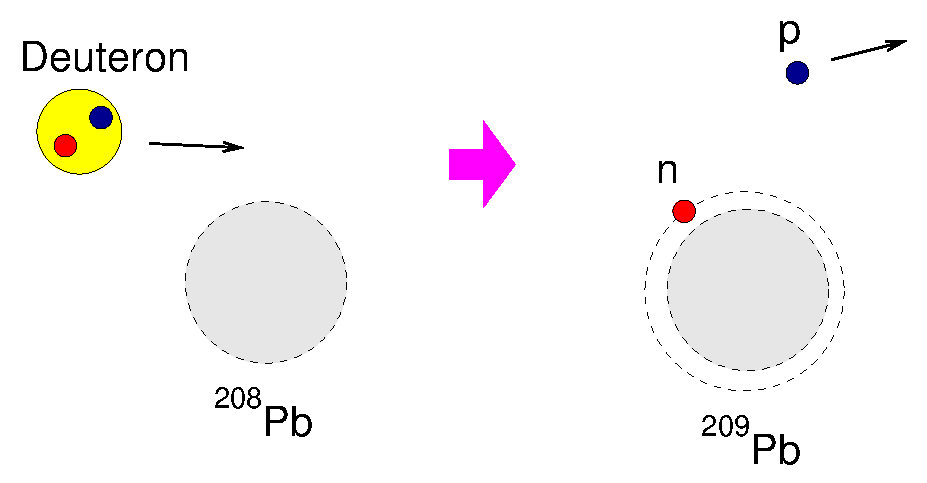
\includegraphics[angle=0]{\images/pb208dp.eps}} \par}
\end{figure}
\end{frame}




% --------------------------------------------------------------------------------------
\begin{comment}
\slide{Transfer reactions: $Q$-value considerations}

{\brick Consider:} $a + A  \rightarrow  b + B$

\begin{itemize}
\gitem{Energy balance (in CM frame):}
$$
\psframebox[linecolor=red,framearc=0.1,framesep=0.1]{
E^{i}_\mathrm{cm} + M_a c^2 + M_A c^2=  E^{f}_\mathrm{cm} +  M_b c^2 +M_B c^2 
}%psframe
$$

\gitem{$Q_0$ value:}
$$
\psframebox[linecolor=red,framearc=0.1,framesep=0.1]{
Q_0= M_a c^2 + M_A c^2 - M_b c^2- M_B c^2
}%psframe
$$

\item[]
$$
\psframebox[linecolor=red,framearc=0.1,framesep=0.1]{
E^{f}_\mathrm{cm} = E^{i}_\mathrm{cm} + Q_0  
}%psframe
$$

\begin{itemize}
\gitem{$Q_0 > 0$}: the system gains kinetic energy (exothermic reaction)
\gitem{$Q_0 < 0$}: the system loses kinetic energy (endothermic reaction)
\end{itemize}
\end{itemize}

\end{frame}


% --------------------------------------------------------------------------------------
\slide{Transfer reactions: $Q$-value considerations}

{\brick Example:} d+\nuc{208}{Pb} $\rightarrow$ p + \nuc{209}{Pb}

\begin{figure}{\par \resizebox*{0.4\textwidth}{!}
{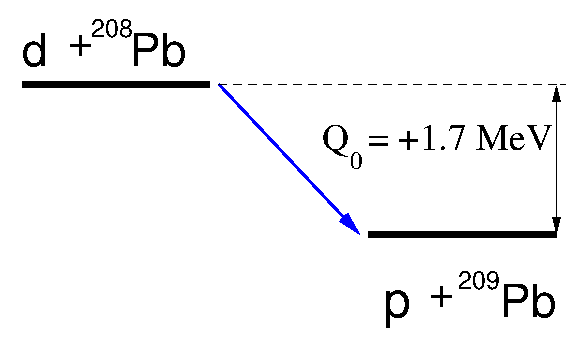
\includegraphics[angle=0]{\images/pb208dp_qvalue.eps}} \par}
\end{figure}

$$
\psframebox[linecolor=red,framearc=0.1,framesep=0.1]{
Q_0= M_d c^2+ M(\mathrm{\nuc{208}{Pb}})c^2 - M_p c^2- M(\mathrm{\nuc{209}{Pb}})c^2 = +1.7 \, \mathrm{MeV}
}%psframe
$$

\medskip
\pause
\ding{43} {\verde $Q_0 > 0$}: the outgoing proton will gain energy with respect to the incident deuteron.

\pause
\bigskip
N.b.: {\small For a transfer reaction, the $Q$ value is just the difference in binding energies of the transferred particle/cluster in the initial and final nuclei:}
$$
Q_0 = \varepsilon_b (f) - \varepsilon_b (i) = 3.936 - 2.224 = +1.7  \, \mathrm{MeV}
$$

\end{frame}

% --------------------------------------------------------------------------------------
\slide{Transfer reactions: $Q$-value considerations}

If the transfer leads to an excited state, the {\verde $Q$-value} will change, and hence the kinetic energy of the outgoing nuclei. 

\begin{figure}{\par \resizebox*{0.5\textwidth}{!}
{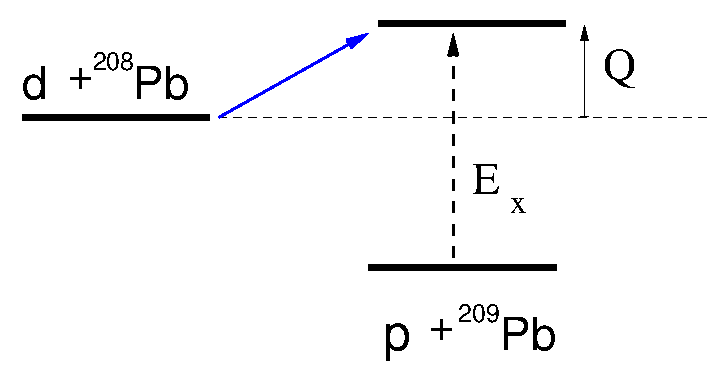
\includegraphics[angle=0]{\images/pb208dp_qvalue_excited.eps}} \par}
\end{figure}

{\bf \verde Energy balance:}
$$
\psframebox[linecolor=red,framearc=0.0,framesep=0.1]{
E^{f}_\mathrm{cm} = E^{i}_\mathrm{cm} + Q =   E^{i}_\mathrm{cm} + Q_0 - E_x 
}%psfrmae
$$

\bigskip
\ding{43}{\em If we know {\verde $Q_0$} we can infer the excitation energies ({\verde $E_x$}) measuring the final kinetic energy of outgoing fragments.}

\end{frame}




% --------------------------------------------------------------------------------------
\slide{What we do observe in a transfer experiment?}


{\verde Example:} d+\nuc{208}{Pb} $\rightarrow$ p + \nuc{209}{Pb}

\begin{figure}{\par \resizebox*{0.8\textwidth}{!}
{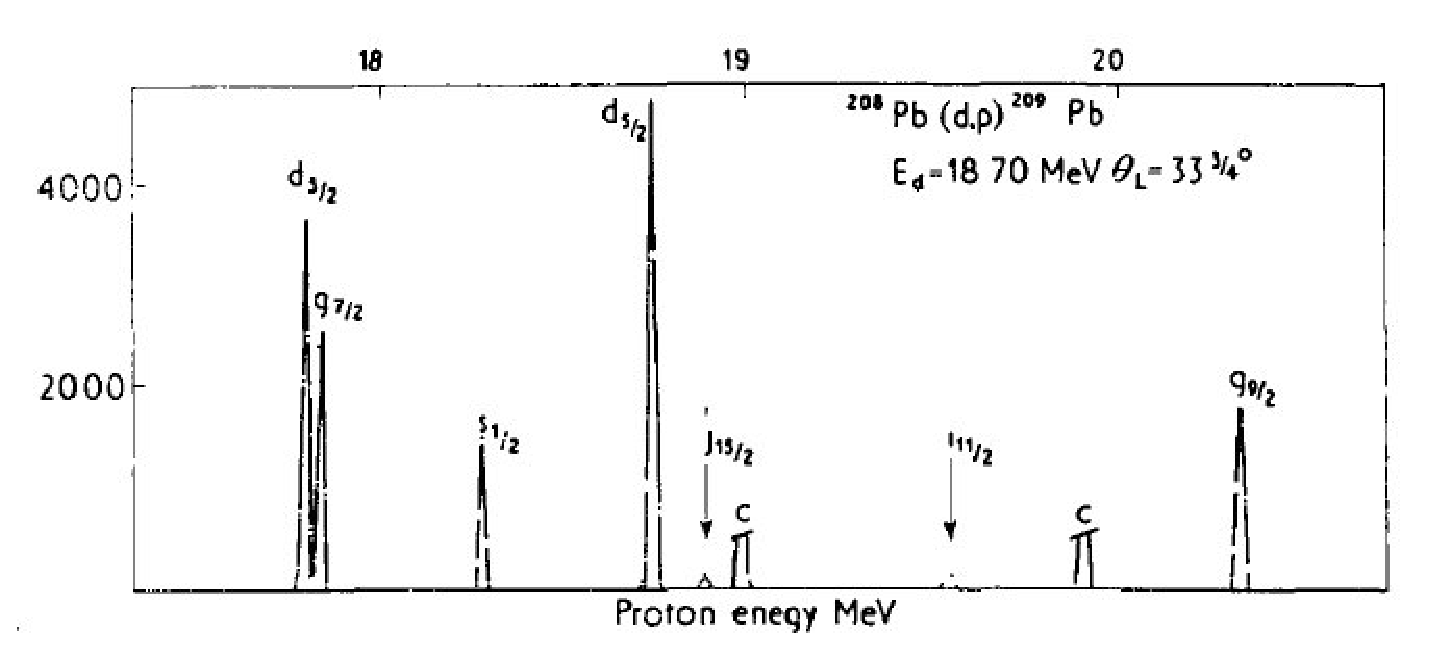
\includegraphics[]{\images/pb208dp_energy.eps}} \par}
\end{figure}

\begin{itemize}
\item[\ding{43}]{\small The proton energy spectrum shows some peaks which reflect the excitation energy spectrum of the residual nucleus (\nuc{209}{Pb})}.
%\item[\ding{43}] Not all the peaks (states) are populated with equal intensity.

\item[\ding{43}] {\small The population probability will depend on the {\blue reaction} dynamics and on the {\blue structure} properties of these states.}
\end{itemize}
\end{frame}




% --------------------------------------------------------------------------------------
\slide{What we do observe in a transfer experiment?}

We would like to infer other properties besides excitation energies:
\begin{itemize}
\item Angular momentum / parity of populated states.
\item Information on the internal structure of these states.
\end{itemize}

\pause 

\begin{center} $\Huge \Downarrow$ \end{center}

\begin{center}\psframebox[linecolor=red,framearc=0.1,framesep=0.1]{\Large \sc SPECTROSCOPY}\end{center} 


\pause 

The excitation function spectrum does not provide in general enough information to extract these properties.
\medskip
 What additional information 
can we use....?

\end{frame}


% --------------------------------------------------------------------------------------
\slide{What we do observe in a transfer experiment?}

\begin{center}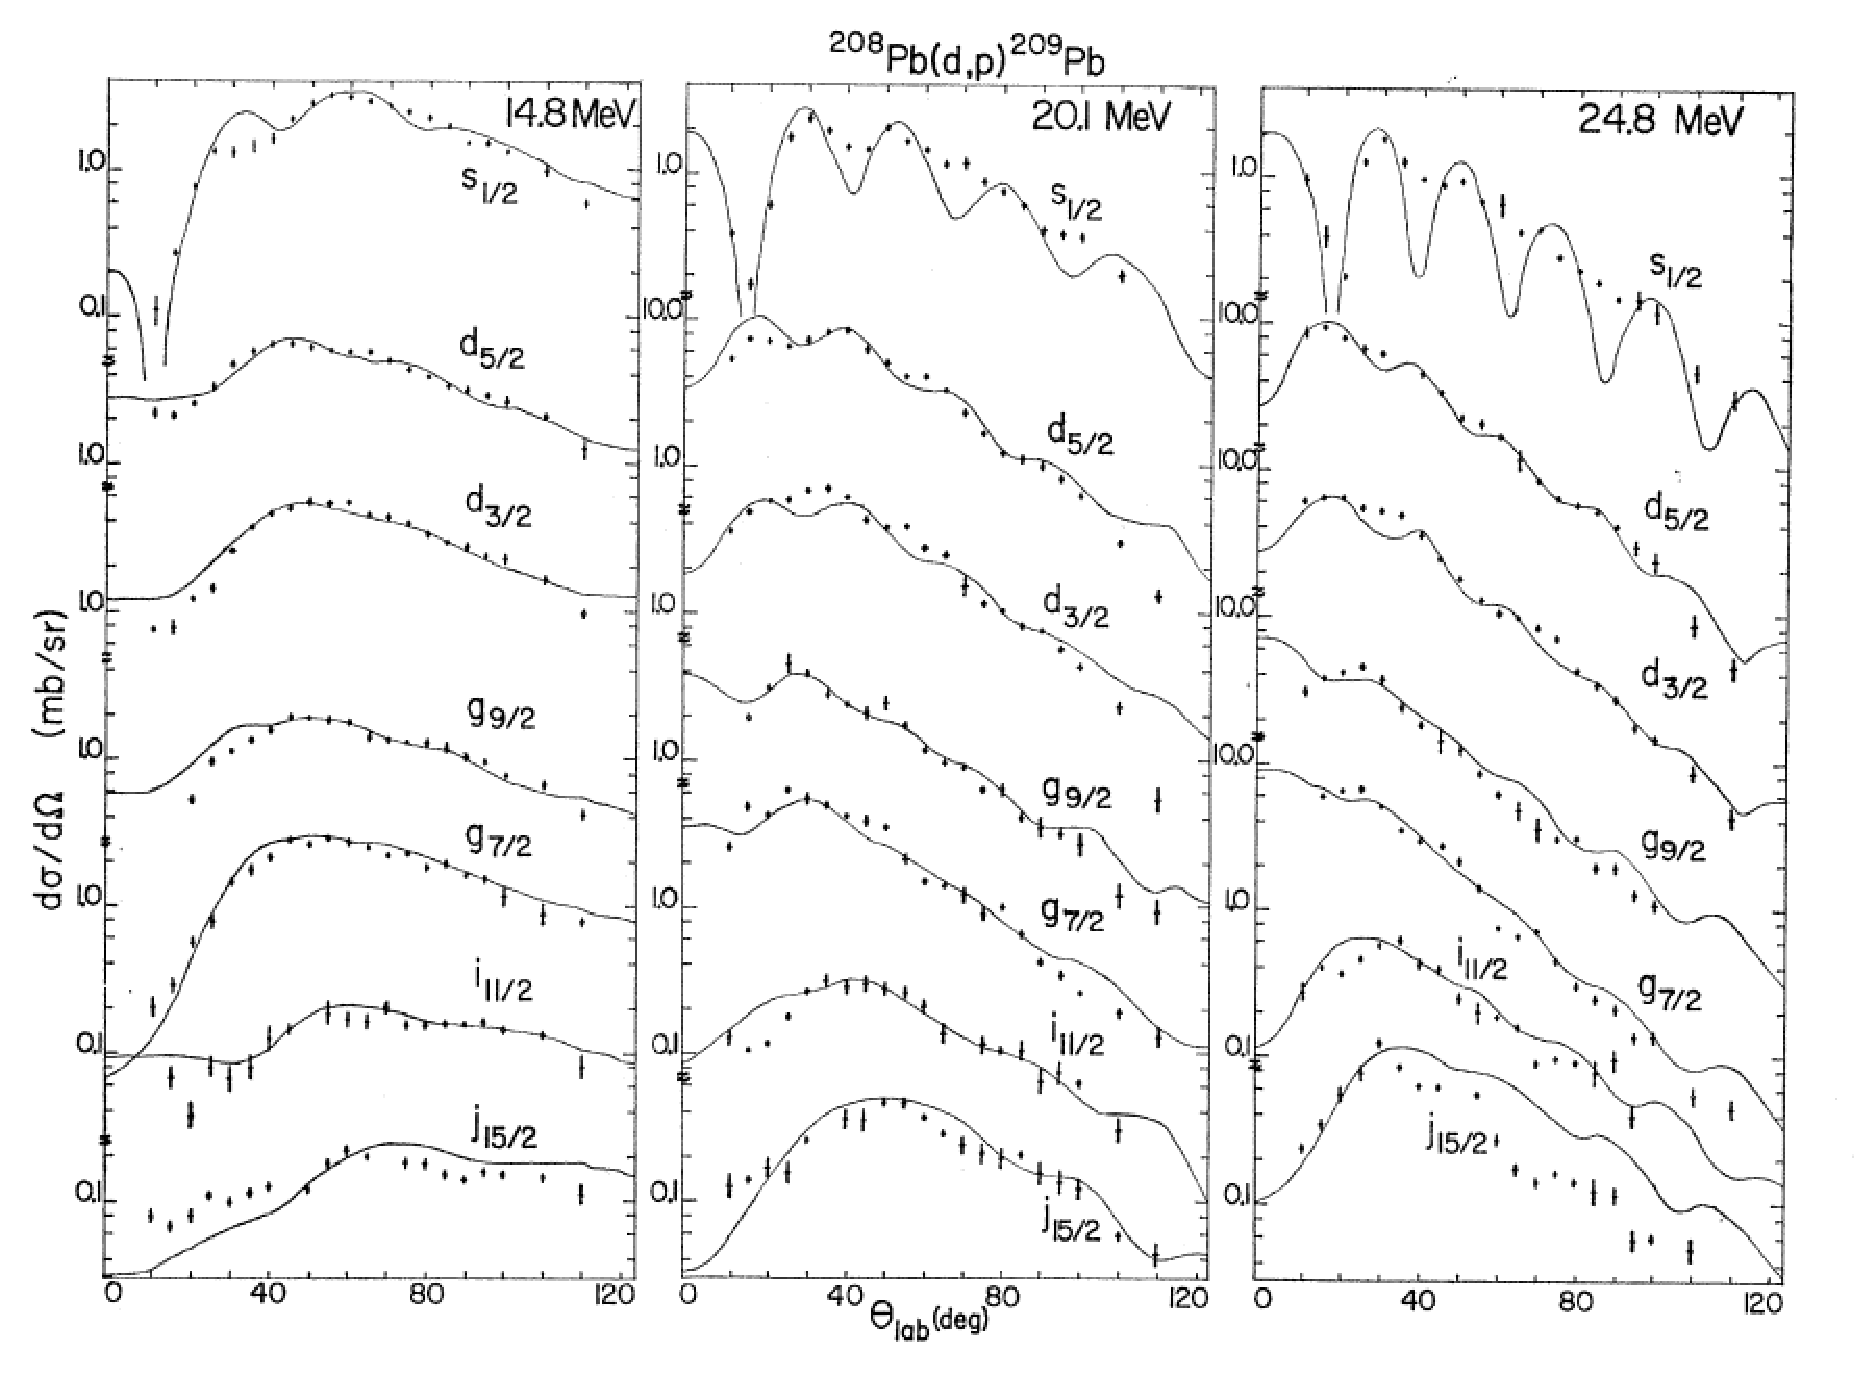
\includegraphics[width=0.7\textwidth]{\images/pb208dp_ang.eps}\end{center}


\ding{43}{\em \verde Angular distributions of transfer cross sections are very sensitive to the internal structure of the populated states} 

\end{frame}


% ----------------------------------------------------------------------------------------------------
\slide{Extracting structure information from transfer reactions}


{\brick Example:} d+\nuc{208}{Pb} $\rightarrow$ p + \nuc{209}{Pb}
\bigskip

\begin{columns}
\column{0.4\linewidth}
%\includegraphics[height=6.5cm]{images/pb208_sp_levels.eps} 
\includegraphics[height=6.5cm]{\images/pb208_sp.eps} 
\column{0.5\linewidth}
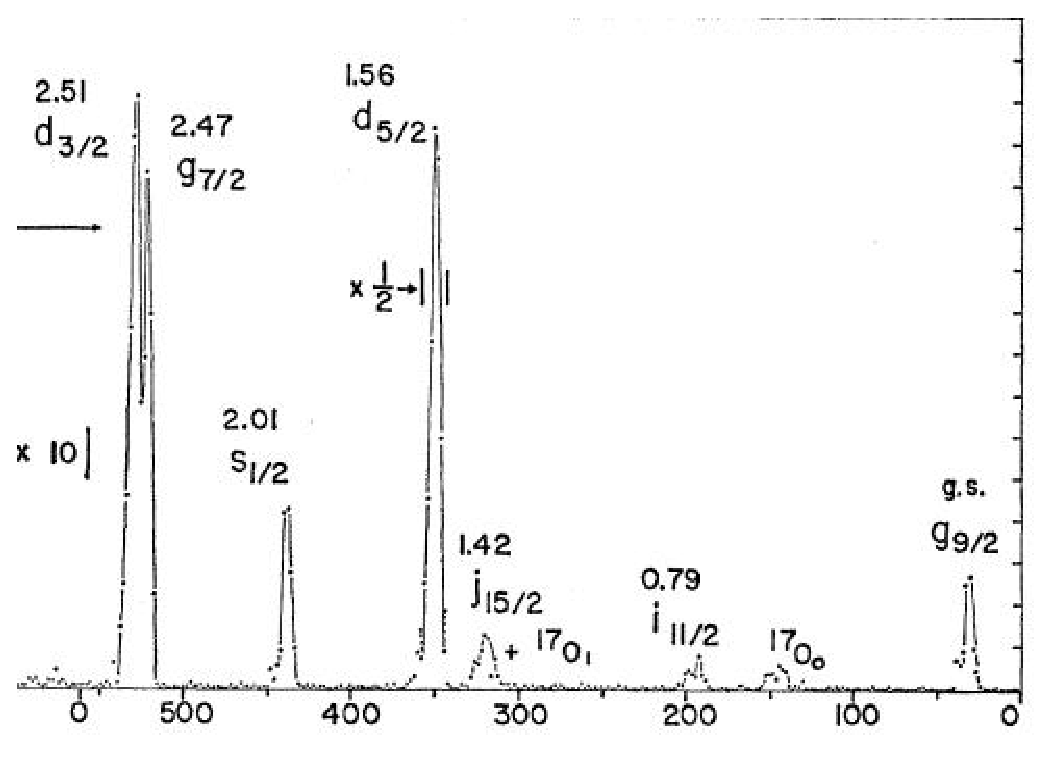
\includegraphics[height=4.5cm]{\images/pb208dp_energy_e20.eps} 

\bigskip

{\verde Phys. Rev. 159 (1967) 1039}
%{\verde Jeans et al, NPA 128 (1969) 224}
\end{columns}%twocolumn


\end{frame}

% ----------------------------------------------------------------------------------------------------
\slide{Extracting structure information from transfer reactions}

 \begin{figure}{\par \resizebox*{0.70\textwidth}{!}
 {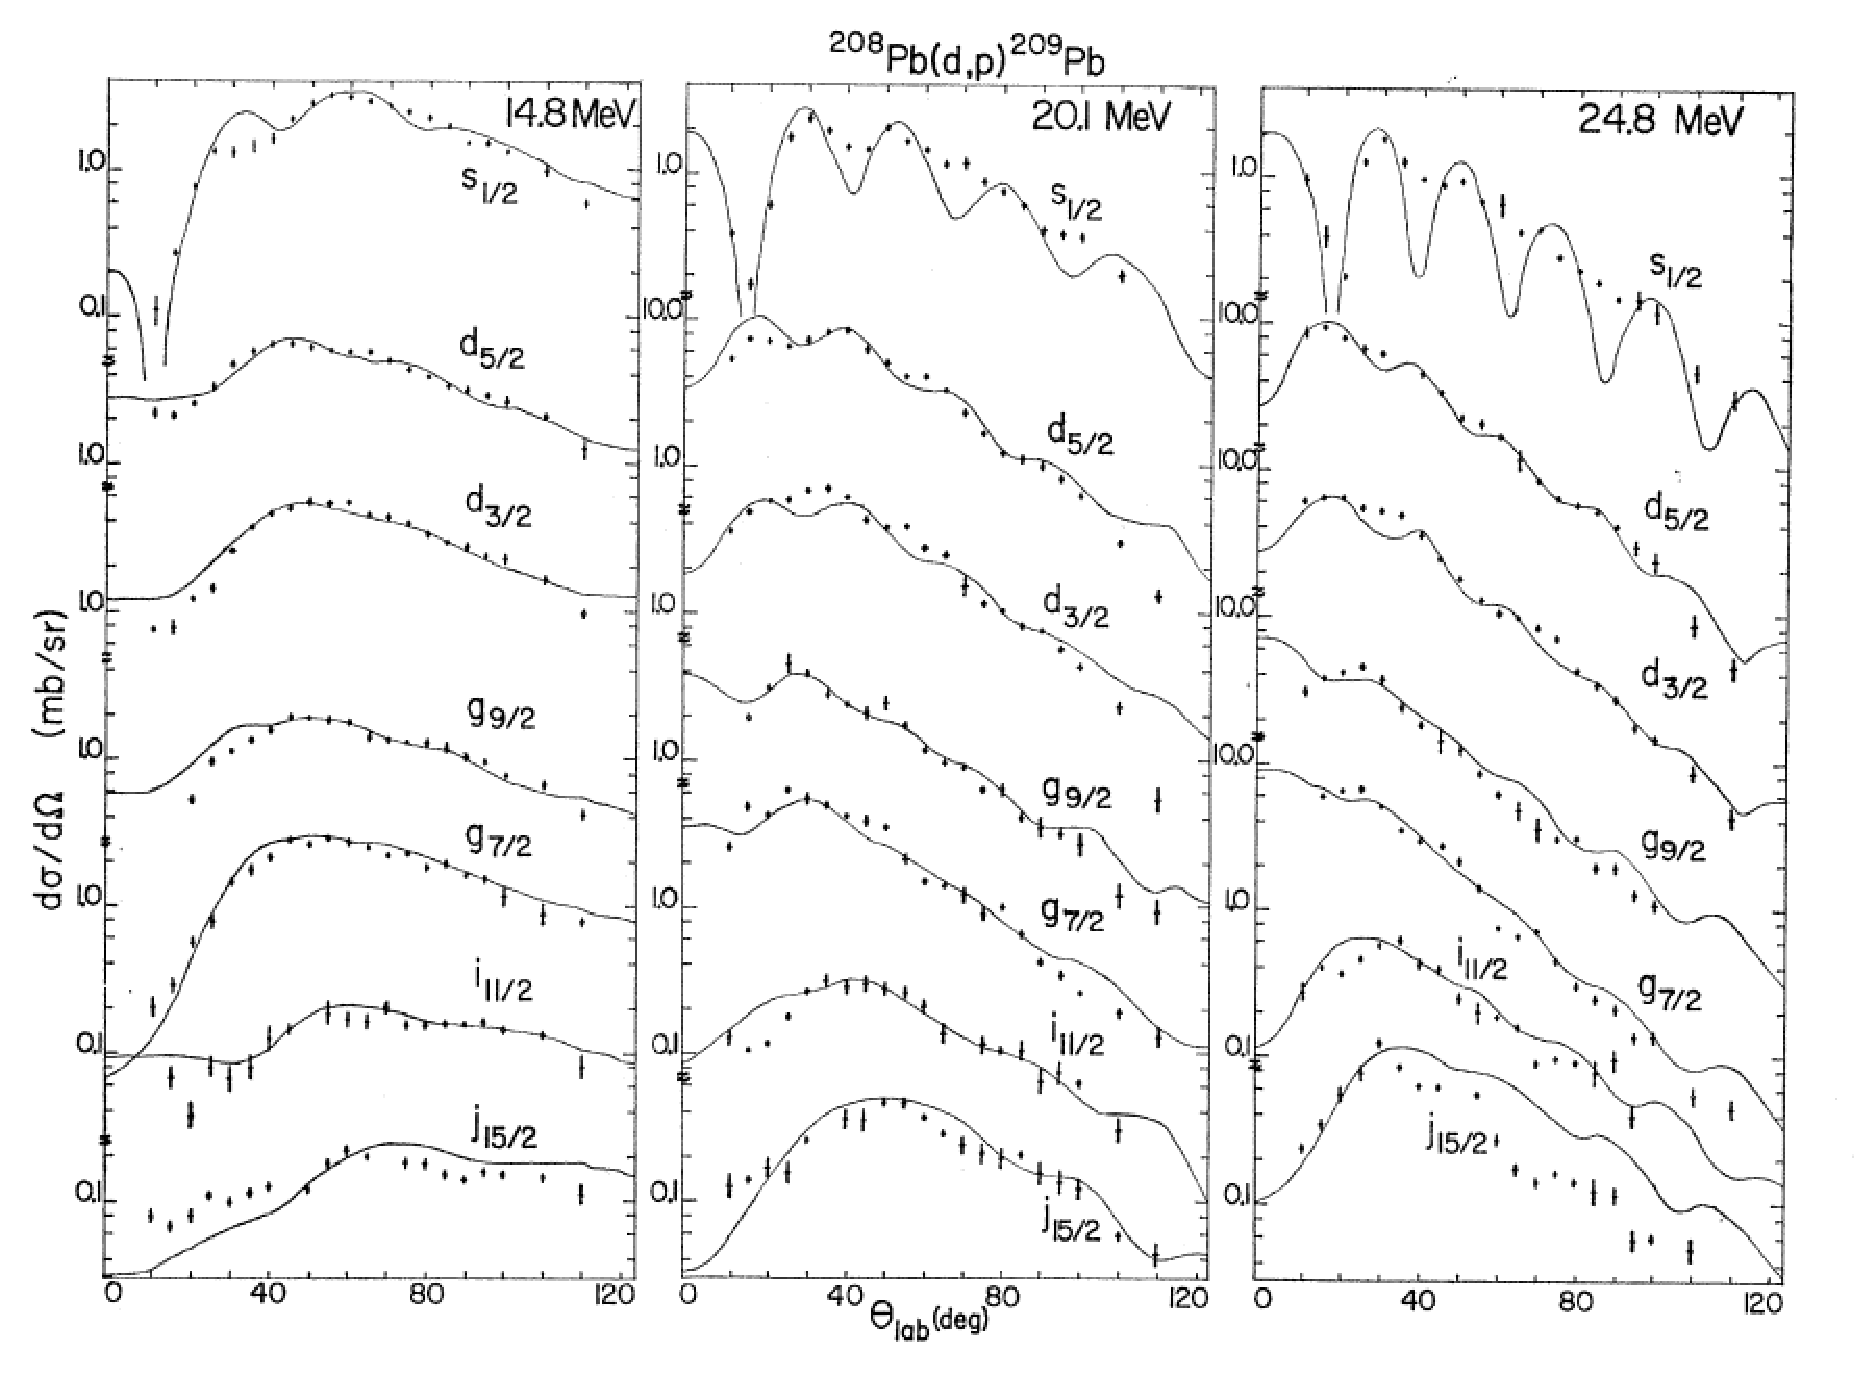
\includegraphics{\images/pb208dp_ang.eps}} \par}
 \end{figure}

\ding{43}{\em \verde Angular distributions of transfer cross sections are very sensitive to the single-particle configuration of 
the transferred nucleon/s.} $\Rightarrow$ $\varphi_{nlj}(\br)$

\end{frame}
\end{comment}



% ----------------------------------------------------------------------------------------------------
\subsection{Formal treatment of transfer reactions}
% ----------------------------------------------------------------------------------------------------
%------------------------------------
\slide{DWBA modelspace}

\begin{figure}{\par \resizebox*{0.35\textwidth}{!}
{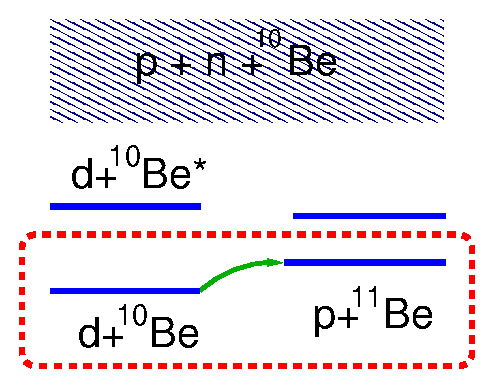
\includegraphics{\images/be10d_modelspace_tr.eps}} \par}
\end{figure}

\vspace{1cm}

\begin{center}
\psframebox[fillcolor=yellow!40,fillstyle=solid,framearc=0.2]{
\parbox{0.8\columnwidth}{%
\ding{43}{\em \small In a transfer calculation, the modelspace will contain states belonging to different mass partitions, and hence to different internal Hamiltonians.}
}%parbox
}%psframe
\end{center}

%\ding{43} In a transfer calculation, the modelspace will contain states belonging to different mass partitions.


\end{frame}




% ----------------------------------------------------------------------------------------------------
\slide{DWBA method for transfer reactions}

\begin{itemize}
\gitem{Transfer process:} $\underbrace{(a+v)}_{A}+b\rightarrow a+\underbrace{(b+v)}_{B}$
%\,\,\,\,(A=a+v,\, B=b+v),$
\begin{figure}{\par \resizebox*{0.5\textwidth}{!}
{\includegraphics{\images/transfer-postprior.eps}} \par}
\end{figure}


\gitem{Full Hamiltonian:} 
 \begin{itemize}
 \setlength{\itemsep}{10pt}
  \item {\blue Prior form:} $\xi_\alpha=\{ \xi, \xi', \br \}$
      $$H = \hat{T}_\bR + H_\alpha(\xi_\alpha) + V_\alpha(\bR,\br) = 
  \hat{T}_\bR + \underbrace{ H_{A}(\xi,\br) + H_b(\xi')}_{H_\alpha(\xi_\alpha)} + \underbrace{ V_{vb}+U_{ab} }_{V_\alpha(\bR,\br)} $$

  \item {\blue Post form:} $\xi_\beta=\{ \xi, \xi', \br' \}$

  $$H = \hat{T}_{\bR'} + H_\beta(\xi_\beta) + V_\beta(\bR',\br')
      = \hat{T}_{\bR'} + \underbrace{ H_{B}(\xi',\br') +
       H_a(\xi)}_{H_\beta(\xi_\beta)} + \underbrace{V_{av}+U_{ab}}_{V_\beta(\bR',\br')} 
$$ 
  \end{itemize}

\end{itemize}
\end{frame}





%-----------------------------------------------------
\slide{The exact transition amplitude}

Scattering amplitude and T-matrix:
% $\alpha \rightarrow \beta$ transition: 
$f_{\beta \alpha}(\theta)= -(\mu_\beta/2 \pi \hbar^2) {\cal T}_{\beta,\alpha}$, with
$$
\psframebox[linecolor=red,framearc=0.1,framesep=0.1]{
{\cal T}^\mathrm{post}_{\beta,\alpha} = 
%{\cal T}^{(0)}_{\beta,\alpha} \delta_{\alpha \beta} +
\int \int \chi_{\beta}^{(-)*}(\bK_\beta, \bR_\beta) 
  \Phi^{*}_\beta (\xi_\beta) (V_\beta-U_\beta)  \Psi^\mathrm{(+)}_{\bK_\alpha}(\bR_\alpha,\xi_\alpha) d\xi_\beta d\bR_\beta 
}%psframe
%{\cal T}^{(exact)}(Ab \rightarrow aB) = 
%\langle \chi^{(-)}_{aB}(\bK',\vec R') \varphi_{bv}(\br') |V_{av}+U_{ab}-U_{aB}|  \Psi^{(+)}_{\bK}(\bR, \br) \rangle .
%}%psframe
$$
\begin{itemize}
\gitem{$\Psi^\mathrm{(+)}_{\bK_\alpha}(\bR_\alpha,\xi_\alpha)$}: exact WF
\gitem{$\Phi_\beta (\xi_\beta)$}: internal (proj + target) WF for final state
\gitem{$\chi_{\beta}^{(+)}(\bK_\beta, \bR_\beta)$}: distorted wave generated by auxiliary potential $U_\beta$
\end{itemize}  


%\item {\verde Outside the range of the potentials:}
%---------------------------------------------------------------------------------------
$$
\small
 \Psi^{(+)}_{\bK_\alpha}(\bR_\alpha,\xi_\alpha) ~  \xrightarrow{R \gg}  
 \underbrace{\vphantom{\sum_{n>0}} e^{i \bK_\alpha \cdot \bR_\alpha} \Phi_\alpha (\xi_\alpha)}_{\mathrm{\blue incident}}   
                  +  \underbrace{\vphantom{\sum_{n>0}} {\red f_{\alpha,\alpha}(\theta)} \frac{e^{i K_\alpha R_\alpha}}{R_\alpha} \Phi_\alpha(\xi_\alpha)}_{\mathrm{\blue elastic}}
                  + \underbrace{\sum_{n>0} {\red f_{\beta,\alpha}(\theta)}  \frac{e^{i K_\beta R_\beta}}{R_\beta}  \Phi_\beta(\xi_\beta)}_{\mathrm{\blue transfer}}
$$

\end{frame}


\slide{Evaluation of scattering amplitude in Born approximation: general case}
\begin{itemize}
\item Define auxiliary potentials in entrance and exit channels: $U_\alpha(\bR_\alpha)$, $U_\beta(\bR_\beta)$ 
\begin{align*}
\left[E-\varepsilon_{\alpha}-\hat{T}_{\bR_\alpha}-U_{\alpha}(\bR_\alpha) \right] \chi^{(+)}_{\alpha}(\bK_\alpha,\bR_\alpha) & =  0 \\
\left[E-\varepsilon_{\beta}-\hat{T}_{\bR_\beta}-U_{\beta}(\bR_\beta) \right] \chi^{(+)}_{\beta}(\bK_\beta,\bR_\beta) & =  0
\end{align*}

\item Retain only elastic component of $\Psi^\mathrm{(+)}_{\bK_\alpha}$  ({\blue Born approximation}):
$$
\Psi^\mathrm{(+)}_{\bK_\alpha} (\bR_\alpha,\xi_\alpha) \approx \chi^{(+)}_{\alpha}(\bK_\alpha,\bR_\alpha) \Phi_\alpha(\xi_\alpha)
$$

\item DWBA scattering amplitude:
$$
\psframebox[fillcolor=magenta!8,linecolor=brick,framearc=0.1,fillstyle=solid]{
{\cal T}^\mathrm{DWBA}_{\beta,\alpha} = 
\int \int \chi_{\beta}^{(-)*}(\bK_\beta, \bR_\beta) 
  \Phi^{*}_\beta (\xi_\beta) (V_\beta-U_\beta)    \chi^{(+)}_{\alpha}(\bK_\alpha,\bR_\alpha) \Phi_\alpha(\xi_\alpha) d\xi_\beta d\bR_\beta 
}%psframe
$$
\end{itemize}
\end{frame}





% ----------------------------------------------------------------------------------------------------
\slide{The important $(d,p)$ case}
\begin{center}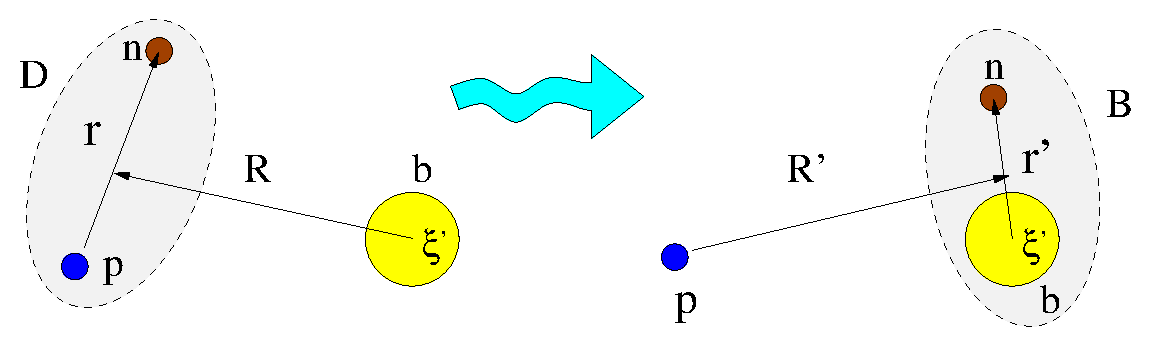
\includegraphics[height=2.0cm]{\images/transfer-dp.eps} \end{center}

 Post-form DWBA transition amplitude: $V_\beta= V_{pn}+ U_{pb}$
$$
\psframebox[fillcolor=magenta!10,linecolor=brick,framearc=0.1,fillstyle=solid]{
{\cal T}^\mathrm{DWBA}_{d,p} = 
\int \int \chi_{p}^{(-)*}(\bK_p, \bR') 
  \Phi^{*}_\beta (\xi_\beta) (V_{pn}+ U_{pb}-U_{pB}) \chi^{(+)}_{d}(\bK_d,\bR) \Phi_\alpha(\xi_\alpha) d\xi_\beta d\bR'
}%psframe
$$

\begin{itemize}
\item For medium-mass/heavy targets: $U_{pb} \approx U_{pB}$ $\Rightarrow$ $V_{pn}+ U_{pb}-U_{pB} \approx V_{pn}(\br)$
\item Internal states and internal coordinates:
\begin{align*}
\Phi_\alpha(\xi_\alpha) & = \varphi_d(\br) \phi_b(\xi')  &    \xi_\alpha= \{ \xi', \br \} \\
\Phi_\beta(\xi_\beta) & =   \Phi_B(\xi',\br')            &   \xi_\beta= \{ \xi', \br' \}
% = {\red C^B_{vb} } \phi_b(\xi') \varphi_{bv}(\br') + \Phi_B^C  
\end{align*}
\end{itemize}
\end{frame}





%------------------------------------------------------------
\slide{$(d,p)$ case: parentage decomposition of target nucleus}

\ding{233} We need to evaluate the {\blue overlap integral}
$$
 \int d\xi' \; \phi^{*}_B (\xi',\br') \phi_b(\xi')    
$$

\ding{233} Use the {\blue parentage decomposition} of $B \rightarrow b + n$ 
$$
\psframebox[linecolor=red,framearc=0.1]{
\phi_{B}^{JM}(\xi,\br)= \sum_{I\ell j}{\verde C_{IJ}^{\ell sj}} \left[\phi_{b}^{I}(\xi)
\otimes 
 {\verde \varphi_{bn}^{\ell sj}(\br)}\right]_{JM}
}%psfr
$$

\begin{itemize}
\gitem{$\varphi_{bn}^{\ell sj}(\br)$:} wavefunction of the valence particle ($n$) relative to the core $b$. 
\gitem{$C_{IJ}^{\ell sj}$} = spectroscopic amplitudes 
\gitem{$S_{IJ}^{\ell sj}=|C_{IJ}^{\ell sj}|^2$} = spectroscopic factors
\end{itemize}

\bigskip
\pause
%\psframebox[linecolor=blue,framearc=0.1,framesep=0.2]{
\ding{43} {\it The spectroscopic factor gives the occupation of the orbital {\red ${\ell sj}$} with the core in  the state with spin {\red $I$}.}
%}%psfr

\ding{43}   $\varphi_{bn}(\br')$ usually approximated by a bound state wfn of $n$ relative to the core $b$.   

\end{frame}





% ----------------------------------------------------------------------------------------------------
\slide{Examples of parentage decompositions}


\begin{enumerate}
\setlength{\itemsep}{13pt}
\gitem{Double-magic nucleus plus a single nucleon:}
$$ 
|\nuc{209}{Bi}(\mathrm{g.s.}) \rangle_{9/2^-}  \approx   
 \left[ |^{208}\mathrm{Pb}(0^+)  \rangle \otimes |\nu 1h_{9/2} \rangle \right]_{9/2^-}
$$

\item[] \ding{43} {\em almost} single-particle configuration ($S_{IJ}^{\ell sj} \approx 1$).

\gitem{Deformed core plus an extra nucleon:} 
$$|^{11}\mathrm{Be}(\mathrm{gs}) \rangle_{1/2^+}  =  
{\red \alpha} \left[ |^{10}\mathrm{Be}(0^+)  \rangle \otimes |\nu 2s_{1/2} \rangle \right]_{1/2^+}+ 
{\red \beta} \left[ |^{10}\mathrm{Be}(2^+)  \rangle \otimes |\nu 1d_{5/2} \rangle \right]_{1/2^+}
+ \ldots   
$$
\item[] with $|\alpha|^2 + |\beta|^2 +\ldots = 1 $
\item The spectroscopic factor reflects the occupation number of a single-particle level so it can be even larger than 1! 

\item There are imporant formal issues related with the non-observability of SF (see works by T.~Duguet and collaborators). 

\end{enumerate}


\end{frame}









%--------------------------------------------------------------------------
\slide{Scattering amplitude and cross sections}

\ding{233} In post form:

$$
\psframebox[fillcolor=magenta!8,linecolor=brick,framearc=0.1,fillstyle=solid]{
{\cal T}^\mathrm{DWBA}_{d,p} =
{\red C^B_{bn} }
\int \int \chi_{p}^{(-)*}(\bK_p, \bR') 
 \varphi^{*}_{bn}(\br') ~V_{pn}(\br) ~ \chi^{(+)}_{d}(\bK_d,\bR) \varphi_{pn}(\br) d\br' d\bR'
}%psframe
$$



$$
\psframebox[fillcolor=magenta!6,linecolor=brick,framearc=0.1,fillstyle=solid]{
\left (\frac{d\sigma}{d\Omega} \right)_{\beta,\alpha} =
\frac{\mu_\alpha \mu_\beta}{(2 \pi \hbar^2)^2}
|{\red C^B_{bn} }|^2
\left | \int \int \chi_{p}^{(-)*}(\bK_p, \bR') 
 \varphi^{*}_{bn}(\br') ~V_{pn}(\br) ~ \chi^{(+)}_{d}(\bK_d,\bR) \varphi_{pn}(\br) d\br' d\bR' \right |^2
}%psframe
$$

$$
{\red |C^B_{bn}|^2 } = {\red S^B_{bn} } = \textrm{spectroscopic factor} 
$$

\begin{center}
\psframebox[fillcolor=yellow!40,fillstyle=solid,framearc=0.2]{
\parbox{0.8\columnwidth}{%
\ding{43}{\em \small  In DWBA, the transfer cross section is proportional to the product of the projectile and target spectroscopic factors. Comparing the data with DWBA calculations, one can extract the values of $ S^B_{bn} $}
}%parbox
}%psframe
\end{center}

\end{frame}






%---------------------------------------------------------------------
\slide{$^1$H($^{11}$Be,$^{10}$Be)$^2$H example}

$$
|^{11}{\rm Be} \rangle  =  {\magenta \alpha} \mid \shalfzero \rangle+ \nonumber 
           {\magenta \beta }\mid \dhalftwo \rangle + \ldots
$$

\ding{233} In DWBA: $$\sigma(0^+) \propto |{\magenta \alpha }|^2  ; \quad  \sigma(2^+) \propto |{\magenta \beta}|^2$$

\pause
%\vspace{0.5cm} 
%\cita{Fortier et al, PLB461, 22 (1999)}
\begin{minipage}[c]{.65\textwidth}
\cita{Fortier et al, PLB461, 22 (1999)}
\begin{center}
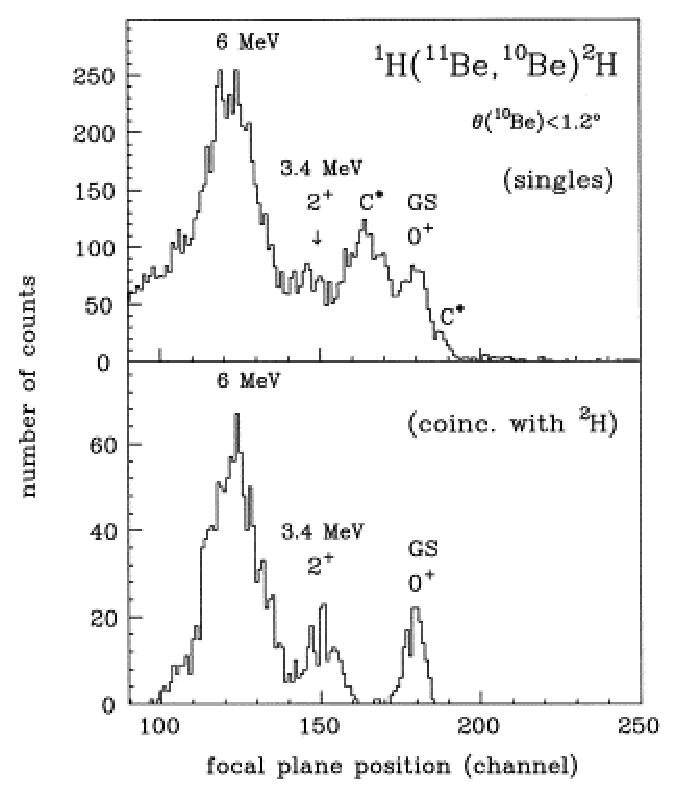
\includegraphics[height=4.5cm]{\images/be11pd_ener.eps} 
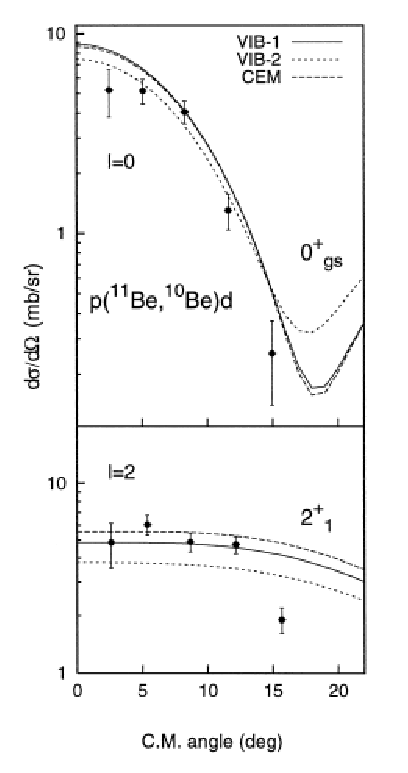
\includegraphics[height=4.5cm]{\images/be11pd_ang.eps} 
\end{center}
\end{minipage}
\begin{minipage}[c]{.25\textwidth}
%\vspace{2cm}
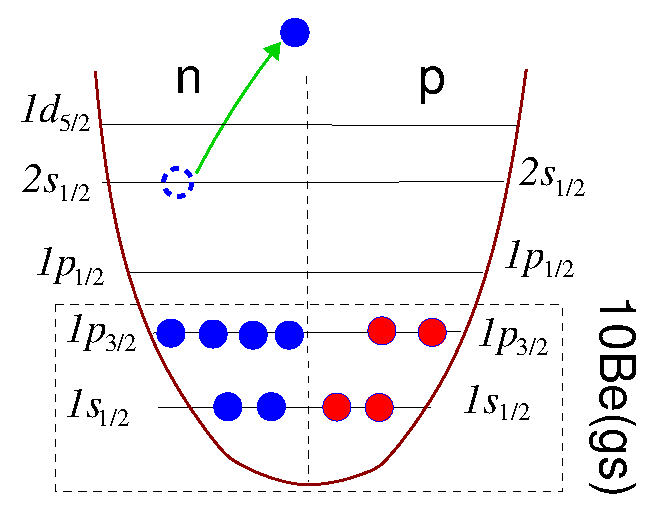
\includegraphics[height=2.0cm]{\images/be11_capas_1ntr.eps} \\
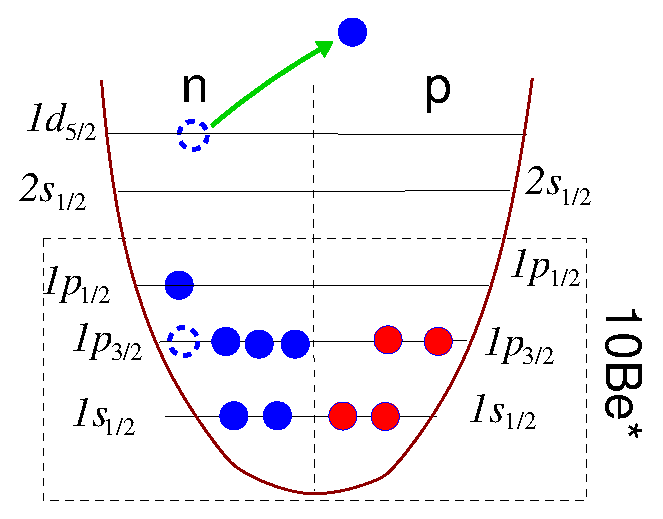
\includegraphics[height=2.0cm]{\images/be11_capas_1ntrex.eps} 
\end{minipage}
\small
\vspace{.5cm}

%\ding{233}{\it  Transfer experiments provide information on the amount of core excitation}

\end{frame}








\begin{comment}

%------------------------------------------
\begin{itemize}
\gitem{Transfer process:} $\underbrace{(a+v)}_{A}+b\rightarrow a+\underbrace{(b+v)}_{B}$
% \begin{figure}{\par \resizebox*{0.5\textwidth}{!}
%{\includegraphics{images/transfer-postprior.eps}} \par}
% \end{figure}

\item If the coupling to the transfer channel is weak, one may write (DWBA):
$$
\psframebox[linecolor=red,framearc=0.1]{
f^\mathrm{prior}_{\beta,\alpha}  = -\frac{\mu_\beta}{2 \pi \hbar^2} \int \int  \widetilde{\chi}_{\beta}^{(-)*}(\bR_\beta) 
\Delta^\mathrm{prior}_{\beta,\alpha}(\bR,\br)
\widetilde{\chi}_{\alpha}^{(+)}(\bR_\alpha)   d\bR_{\alpha} d \br
}%psframebox
$$

\item[] with the {\blue coupling potential}:
$$ 
\psframebox[linecolor=red,framearc=0.1]{
\Delta^\mathrm{prior}_{\beta,\alpha}(\bR,\br)=
\int d\xi d\xi' \; \phi_a(\xi) \phi_B (\xi',\br') 
{\mathbf \Delta}_\mathrm{prior}(\bR,\br) \phi_A (\xi,\br) \phi_b(\xi') 
}%psframe
$$

\end{itemize}

\end{frame}

\end{comment}









%\subsection{The $(d,p)$ reaction}





% ------------------------------------------------------------------------------------------------
\slide{Beyond DWBA: CCBA formalism}

In presence of strongly coupled excited states in the initial or final partition, the CC and DWBA formalisms
can be combined $\rightarrow$ {\blue CCBA}

 \begin{figure}{\par \resizebox*{0.3\textwidth}{!}
 {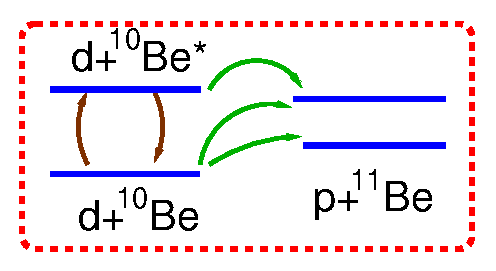
\includegraphics{\images/be10d_modelspace_ccba.eps}} \par}
 \end{figure}


Exact scattering amplitude ({\it post form}): ($\beta \neq \alpha$)
$$
\psframebox[linecolor=red,framearc=0.1,framesep=0.1]{
{\cal T}^\mathrm{post}_{\beta,\alpha} = 
\int \int \chi_{\beta}^{(-)*}(\bK_\beta, \bR_\beta) 
  \Phi^{*}_\beta (\xi_\beta) (V_\beta-U_\beta)  \rnode{F1}{\underbrace{\Psi^\mathrm{(+)}_{\bK_\alpha}(\bR_\alpha,\xi_\alpha)}} d\xi_\beta d\bR_\beta 
}%psframe
$$

$$
\rnode{T1}{
\psframebox[linecolor=red,framearc=0.1,framesep=0.1]{
\Psi^\mathrm{(+)}_{\bK_\alpha}(\bR_\alpha,\xi_\alpha) \approx \Psi^\mathrm{CC}_{\bK_\alpha}(\bR,\xi) =
\phi_{0}(\xi)\chi_{0}(\bR)+ \sum_{n>0} \phi_{n}(\xi)\chi_{n}(\bR)
}%psframe
}%rnode
$$
{\nccurve[linecolor=blue,angleA=-90,angleB=90]{->}{F1}{T1}}

\end{frame}



% ------------------------------------------------------------------------------------------------
\slide{Beyond DWBA: CCBA formalism}

When there are strongly coupled excited states in the initial or final partition, the CC and DWBA formalisms
can be combined $\rightarrow$ {\blue CCBA}

\bigskip

\only<1>{
% \twocolumn{
 {\bf Ej:} \nuc{172}{Yb}(p,d) {\verde Ascuitto et al, Nucl Phys. A226 (1974) 454} 
% }{
 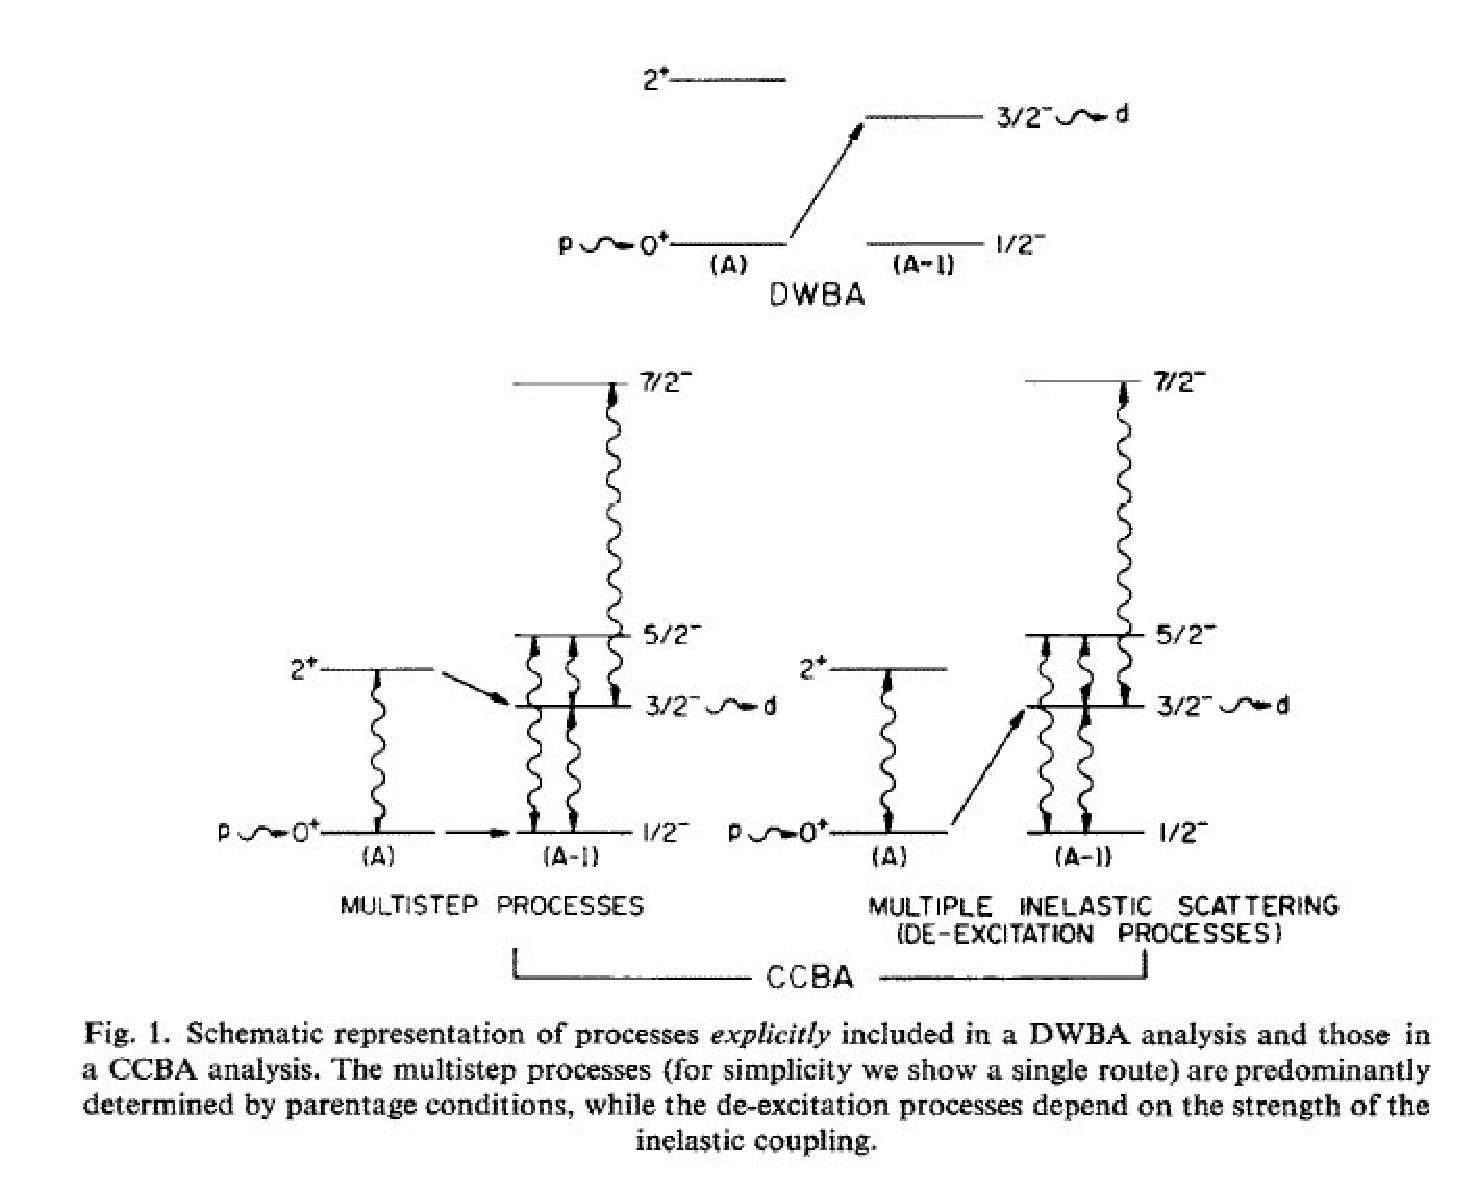
\includegraphics[width=0.65\textwidth]{\images/yb172pd_ccba_scheme.eps}
% }%twocolumn
}
\only<2>{
 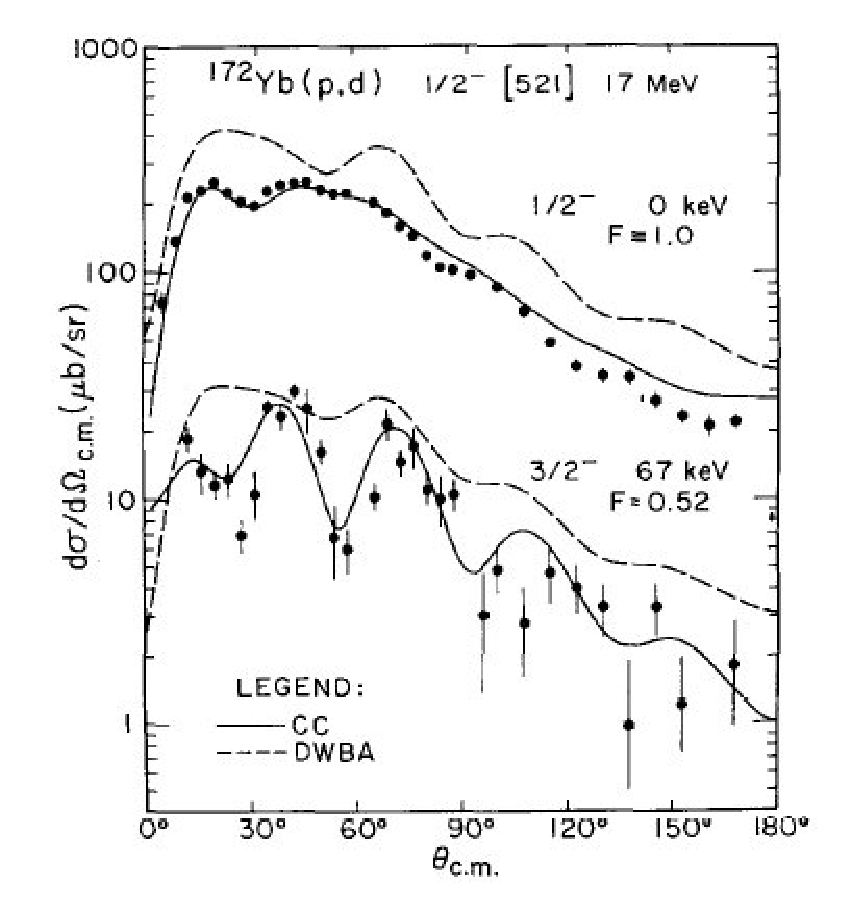
\includegraphics[width=0.4\textwidth]{\images/yb172pd_ccba.eps}
 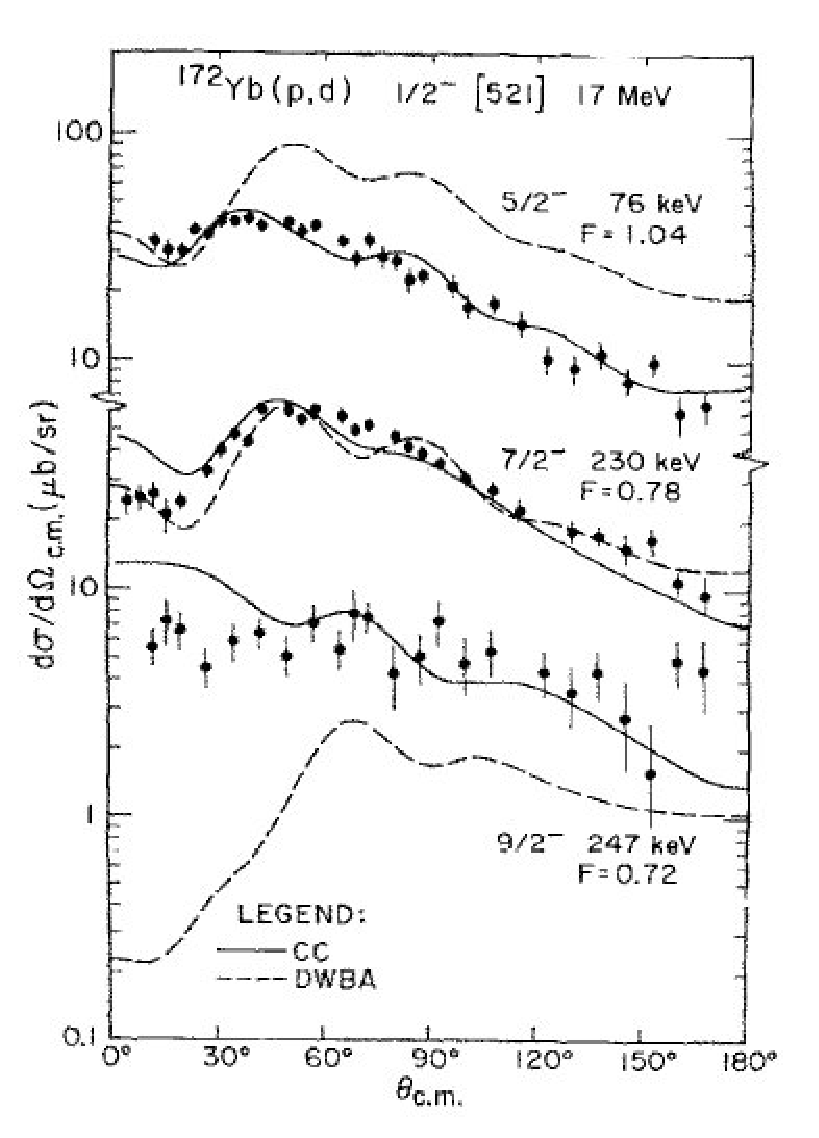
\includegraphics[width=0.4\textwidth]{\images/yb172pd_ccba2.eps}
}
\end{frame}


%---------------------------------------------------------
\subsection{Transfer reactions with weakly bound nuclei}
%---------------------------------------------------------
\slide{}
\begin{center}
\psframebox[fillcolor=green!10,linecolor=blue,framearc=0.1,fillstyle=solid,framesep=5pt]{
Transfer reactions with weakly bound nuclei
}%psframe
\end{center} 
\end{frame}



%-----------------------------------------------------------
\slide{Transfer reactions with weakly bound nuclei}

\begin{itemize}
\item DWBA approximates the total WF by the elastic channel and assumes that transfer occurs in one step (Born approximation). 

\item For weakly bound projectiles (eg.~deuterons), breakup is an important channel and can influence the transfer process. 

 \begin{figure}{\par \resizebox*{0.3\textwidth}{!}
 {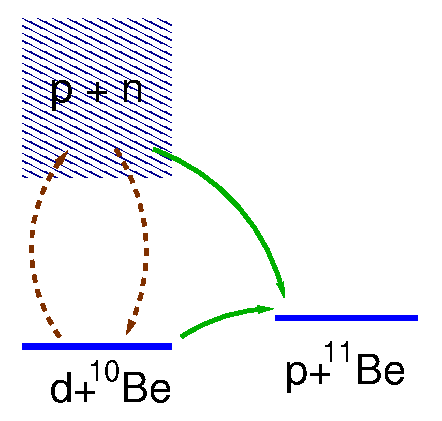
\includegraphics{\images/be10dp_channels_dbu.eps}} \par}
 \end{figure}


\item $\Psi^\mathrm{(+)}_{\bK_d}(\bR,\br)$ includes breakup components, but these are lost when we make the DWBA approximation ($\Psi^\mathrm{(+)} \approx \chi^{(+)}_{d}(\bK_d,\bR) \varphi_{d}(\br)$)  $\Rightarrow$ need to go beyond DWBA 
\end{itemize}

\end{frame}


%-----------------------------------------
\slide{Zero-range and Finite-range adiabatic approximations (ADWA)}
\begin{itemize}
\item For the transfer matrix element, we need only $\Psi^\mathrm{(+)}_{\bK_d}(\bR,\br)$ for small $|\br|$

\item {\blue Zero-range} approximation : $\chi^{ad}_d(\bR,\br) \simeq \chi^{ad}_d(\bR,0) \equiv \chi^{JS}_d(\bR)$
$$
\psframebox[linecolor=red,framearc=0.1]{
[\hat{T}_\bR + \varepsilon_d + U^{JS}(R) - E]  \chi^{JS}_d(\bR) =0 
}
\quad 	\textrm{(Johnson-Soper)}
$$ 
$$ 
\psframebox[linecolor=red,framearc=0.1]{
U^{JS}(R) =U_{pb}(R)  + U_{nb} (R)
}%psframe
$$

\item Or, with {\blue finite-range} corrections :
$$
\psframebox[linecolor=red,framearc=0.1]{
U^{JT}(R)=  \frac{\langle \varphi_{pn}(\br) | V_{pn} (U_{nb}+U_{pb}) | \varphi_{pn}(\br) \rangle}{\langle \phi_{pn}(\br) | V_{pn} | \phi_{pn}(\br) \rangle} 
}%psframe
\quad 
\textrm{(Johnson--Tandy)}
$$

\end{itemize}
\end{frame}


%--------------------------------------------------------
\slide{CDCC-BA approximation}

\bi
\item Recall the exact transition amplitude:

$$
\psframebox[linecolor=red,framearc=0.1,framesep=0.1]{
{\cal T}^\mathrm{post}_{\beta,\alpha} = 
%{\cal T}^{(0)}_{\beta,\alpha} \delta_{\alpha \beta} +
\int \int \chi_{\beta}^{(-)*}(\bK_\beta, \bR_\beta) 
  \Phi^{*}_\beta (\xi_\beta) (V_\beta-U_\beta) 
\rnode{F1}{\underbrace{\Psi^\mathrm{(+)}_{\bK_\alpha}(\bR_\alpha,\xi_\alpha)}} d\xi_\beta d\bR_\beta 
}%psframe
$$


\item Use CDCC approximation for $\Psi^\mathrm{(+)}_{\bK_\alpha}$:
$$
\rnode{T1}{\Psi^\mathrm{(+)}_{\bK_\alpha}} \approx \Psi^\mathrm{CDCC}
= 
\underbrace{\chi_0(\bK_\alpha,\bR)\phi_0(\br)}_{\mathrm{\blue elastic}} 
 + \sum_{n',j,\pi} 
\underbrace{\phi^{j\pi}_{n'}(k_{n'},\br) \chi_{n',j,\pi}(\bK_{n'},\bR)}_{\mathrm{\blue breakup}} 
$$
 
{\nccurve[linecolor=blue,angleA=-90,angleB=90]{->}{F1}{T1}}


\end{itemize}


%---------------------------------------------------------------------------------------
%$$
%\small
% \Psi^{(+)}_{\bK_\alpha}(\bR_\alpha,\xi_\alpha) ~  \xrightarrow{R \gg}  
% \underbrace{\vphantom{\sum_{n>0}} e^{i \bK_\alpha \cdot \bR_\alpha} \Phi_\alpha (\xi_\alpha)}_{\mathrm{\blue incident}}   
%                  +  \underbrace{\vphantom{\sum_{n>0}} {\red f_{\alpha,\alpha}(\theta)} \frac{e^{i K_\alpha R_\alpha}}{R_\alpha} \Phi_\alpha(\xi_\alpha)}_{\mathrm{\blue elastic}}
%                  + \underbrace{\sum_{n>0} {\red f_{\beta,\alpha}(\theta)}  \frac{e^{i K_\beta R_\beta}}{R_\beta}  \Phi_\beta(\xi_\beta)}_{\mathrm{\blue transfer}}
%$$




\end{frame}


%--------------------------------------------------------
\slide{DWBA, ADWA and CDCC-BA compared}
\begin{center}
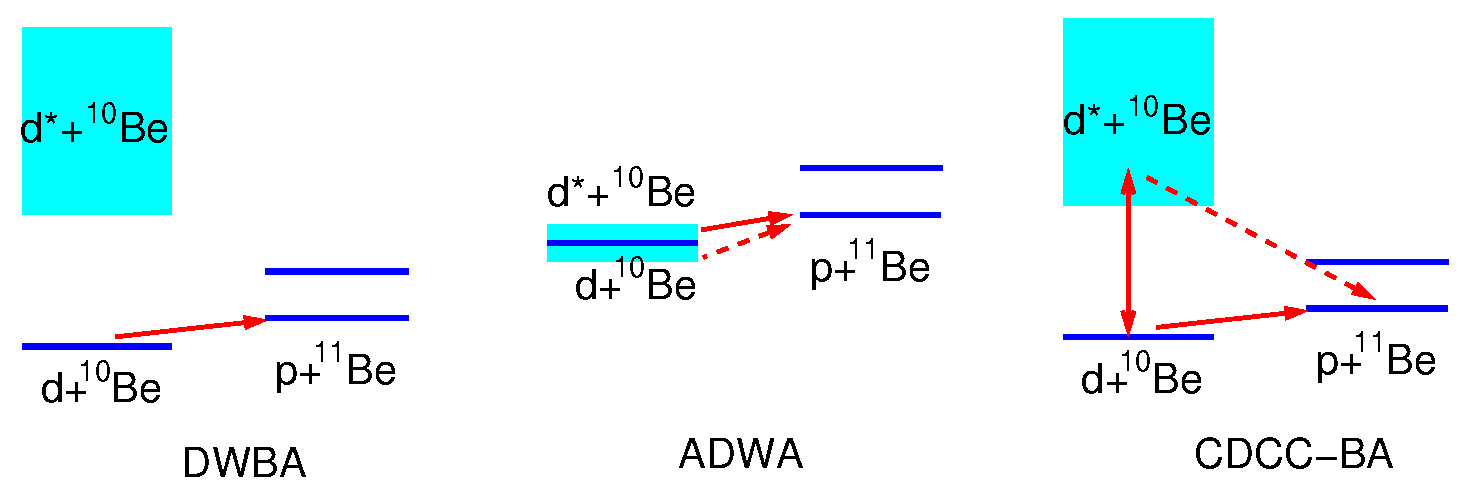
\includegraphics[width=0.75\textwidth]{\images/be10dp_schemes.eps}
\end{center}

\end{frame}



% ----------------------------------------------------------------------------------
\subsection{Accessing continuum structures by transfer reactions}


%----------------------------Shell evolution for N=7 --------------
\slide{Shell evolution with neutron/proton asymmetry}

\ding{233}{\small Systematic studies of shell evalution requires extensions to the continuum}
%The extracted positions for the $s_{1/2}$ virtual state and $p_{1/2}$ resonances constitute a clear evidence of the parity inversion of these two levels for $N \gg Z$ isotopes}

\begin{columns}
\column{0.35\textwidth}
\begin{center} 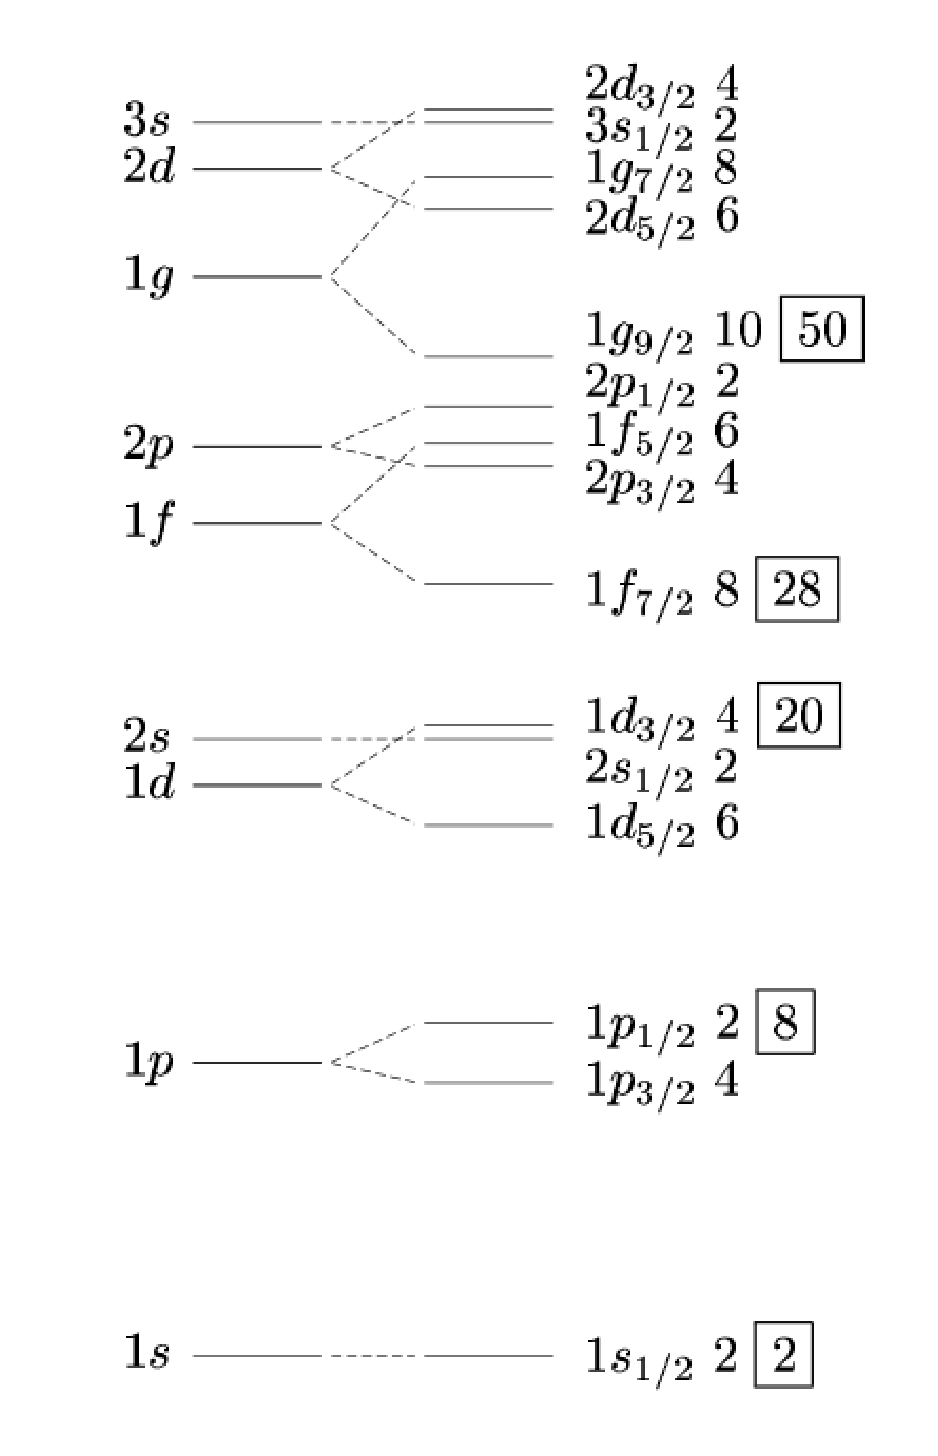
\includegraphics[width=0.8\columnwidth]{\images/Shells.eps} \end{center}
\column{0.65\textwidth}
\begin{center} Shell-evolution for N=7 isotones \end{center}
\begin{center}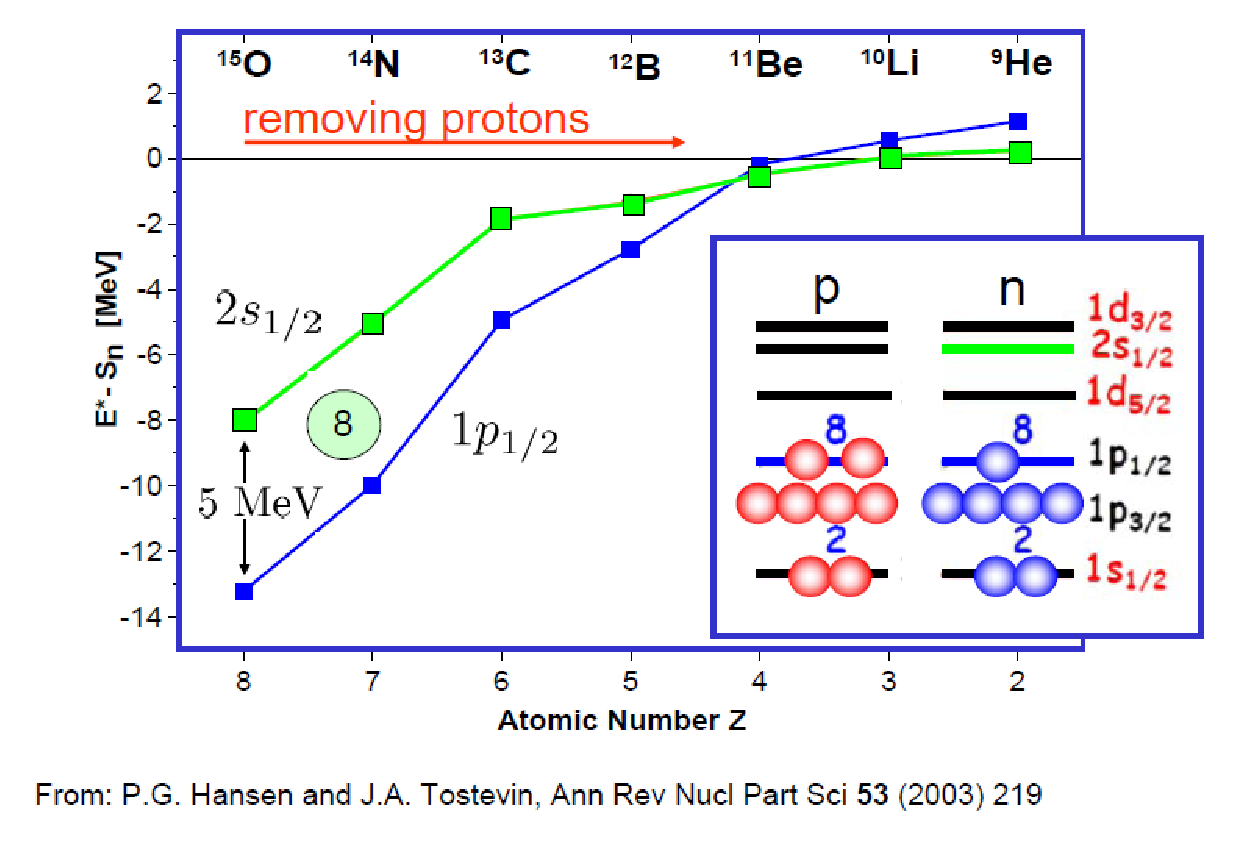
\includegraphics[width=0.95\columnwidth]{\images/n7_sp.eps} \end{center}
{\small SM explanation: Otsuka et al, PRL95,232502(2005)}
\end{columns}
\end{frame}


% ---------------------------------------------------------------------------------------------------
\slide{Spectroscopy in the continuum: the $^{10}$Li case }

%Eg.~Studying the continuum of $^{10}$Li$^*$ via  $^{9}$Li+d $\rightarrow$ p + $^{9}$Li+n

%\mishadowbox{\sc \brick nBest fit results:} {\verde HP.Jeppesen et al, PLB642 (2006) 449}

%\begin{itemize}
%\setlength{\itemsep}{4pt}
%\item {\blue $p_{1/2}$ resonance} (1$^+$ or 2$^+$ ): {\verde $E_r \simeq 0.38$~MeV, $\Gamma=0.2$~MeV}
%\item {\blue $s_{1/2}$ virtual state} (1$^-$ or 2$^-$): {\verde $a_s \simeq-24$~fm} 
%\end{itemize}

\ding{43} Detected protons carry information on the $^{9}$Li+n excitation spectrum. 
\medskip

\begin{columns}
\column{0.5\textwidth}
 \psframebox[linecolor=red,framearc=0.25,framesep=0.1]{
 \parbox{4.5cm}{
  \begin{center}
% {\blue Direct mechanism} 
 \end{center}
\vspace{-0.5cm}
\begin{figure}{\par \resizebox*{0.45\columnwidth}{!}
{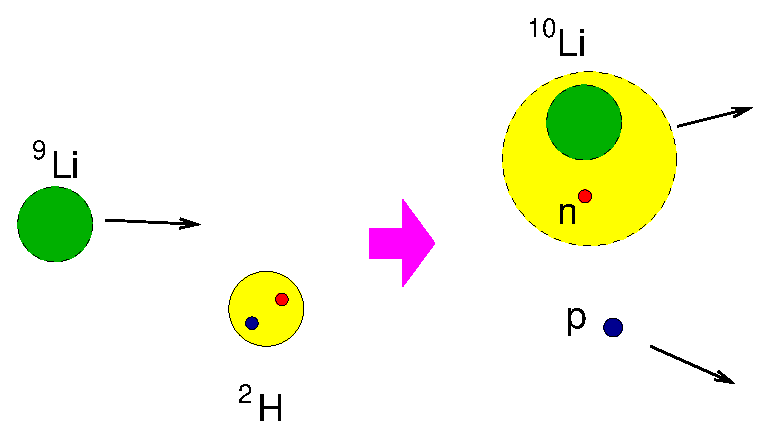
\includegraphics{\images/10li-trans.eps}} \par}
\end{figure}
%\centering{CCBA with unbound states}
 \begin{figure}{\par \resizebox*{0.45\columnwidth}{!}
 {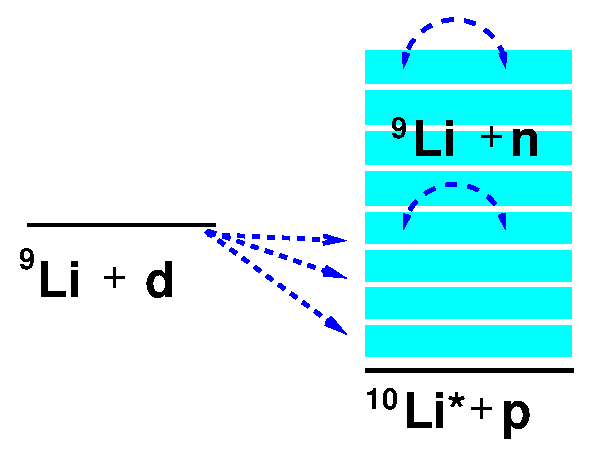
\includegraphics{\images/li9dp_ccba.eps}} \par}
\end{figure}

}%parbox
}%psframebox

\column{0.53\textwidth}
\begin{center}
\cita{H.P.~Jeppesen et al, PLB642 (2006) 449}
\end{center}
\begin{figure}{\par \resizebox*{0.9\textwidth}{!}
{\includegraphics{\images/bu_vsE_data.eps}} \par}
\end{figure}
%\scriptsize
%\begin{itemize}
%\setlength{\itemsep}{4pt}
%\item {\blue $p_{1/2}$ resonance} (1$^+$ or 2$^+$ ): {\verde $E_r \simeq 0.38$~MeV, $\Gamma=0.2$~MeV}
%\item {\blue $s_{1/2}$ virtual state} (1$^-$ or 2$^-$): {\verde $a_s \simeq-24$~fm} 
%\end{itemize}
\end{columns}


% \vspace{-0.25cm}
% \twocolumn{
% \begin{figure}{\par \resizebox*{0.45\textwidth}{!}
% {\includegraphics{10li-trans-cm.eps}} \par}
% \end{figure}
% }{
% %{\verde \em \small We are observing the tail of the proton angular distribution!}
%  }

\end{frame}




%---------------------------------------------------------------------------------------------
\slide{Spectroscopy to unbound states: \nuc{9}{Li}(d,p)\nuc{10}{Li} case}

\begin{center}{\blue \psframebox[fillcolor=yellow]{$p_{1/2}$ resonance}}\end{center}

\bc
\column{0.5\textwidth}
\begin{figure}{\par \resizebox*{0.9\textwidth}{!}
{\includegraphics{figs/li9nn_pshift_p12}} \par}
\end{figure}

\psframebox[fillcolor=yellow,linecolor=red,framearc=0.1]{
\parbox{4.5cm}{
\begin{itemize}
\setlength{\itemsep}{10pt}
\item[$\bullet$] {\blue $E_\mathrm{res} \to \delta(E_\mathrm{res})=\frac{\pi}{2}$} 
\item[$\bullet$] {\blue $\frac{2}{\Gamma}= \frac{d\delta}{dE}$}
\end{itemize}
}%parbox
}%frame
\column{0.5\textwidth}
\begin{figure}{\par \resizebox*{0.9\textwidth}{!}
{\includegraphics{figs/p12res.eps}} \par}
\end{figure}
\ec
\end{frame}



%----------------------------------------------------
\slide{Spectroscopy to unbound states: \nuc{9}{Li}(d,p)\nuc{10}{Li} case}

\bc
\column{0.5\textwidth}
\begin{center}
\rnode{bi}{\brick \blue \psframebox{Structure: $p_{1/2}$ resonance}}
\end{center}
\vspace{-0.5cm}
\only<1>{
\begin{figure}{\par \resizebox*{0.8\textwidth}{!}
{\includegraphics{figs/p12res-v66.eps}} \par}
\end{figure}
}%onslide
\only<2>{
\begin{figure}{\par \resizebox*{0.8\textwidth}{!}
{\includegraphics{figs/p12res-v66.5.eps}} \par}
\end{figure}
}%onslide
\only<3>{
\begin{figure}{\par \resizebox*{0.8\textwidth}{!}
{\includegraphics{figs/p12res-v67.eps}} \par}
\end{figure}
}%onslide
%
\column{0.5\textwidth}
\begin{center}
\rnode{bf}{\blue \psframebox{Reaction}}
\end{center}
\vspace{0.25cm}
\only<1>{
\begin{figure}{\par \resizebox*{1.00\textwidth}{!}
{\includegraphics{figs/bu_vsE_p12_v66.eps}} \par}
\end{figure}
}%onslide
\only<2>{
\begin{figure}{\par \resizebox*{1.00\textwidth}{!}
{\includegraphics{figs/bu_vsE_p12_v66.5.eps}} \par}
\end{figure}
}%onslide
\only<3>{
\begin{figure}{\par \resizebox*{1.00\textwidth}{!}
{\includegraphics{figs/bu_vsE_p12_v67.eps}} \par}
\end{figure}
}%onslide
\ec
\ncline[linecolor=red]{->}{bi}{bf}
\end{frame}



%-------------------------------------------------------------------------
\slide{Spectroscopy of unbound states: \nuc{9}{Li}(d,p)\nuc{10}{Li} case}

\begin{columns}
\column{0.5\linewidth}
\begin{center}
\rnode{bi}{\brick \blue \psframebox{$V_p$(resonance)}}
\end{center}
\vspace{-0.5cm}
\begin{figure}{\par \resizebox*{0.8\textwidth}{!}
{\includegraphics{figs/p12res.eps}} \par}
\end{figure}
%
\column{0.5\linewidth}
\begin{center}
\rnode{bf}{\blue \psframebox{Reaction}}
\end{center}
\vspace{0.25cm}
\begin{figure}{\par \resizebox*{1.00\textwidth}{!}
{\includegraphics{figs/bu_vsE_p12_vdep.eps}} \par}
\end{figure}
\end{columns}

\ncline[linecolor=red]{->}{bi}{bf}

\end{frame}







%----------------------------------------------------------------------------
\slide{Spectroscopy to unbound states: \nuc{9}{Li}(d,p)\nuc{10}{Li} case}

\begin{columns}
\column{0.5\linewidth}
\begin{center}
\rnode{ai}{\brick \blue \psframebox[fillcolor=yellow]{Structure: $s_{1/2}$ virtual state}}
$$V^{(s)}_{nc}(r)=-V_{s} \exp(-r^2/a^2) \quad (a=2~\mathrm{fm})$$
\end{center}
\vspace{-0.5cm}
\only<1>{
\begin{figure}{\par \resizebox*{0.8\textwidth}{!}
{\includegraphics{\images/slength3_v90.eps}} \par}
\end{figure}
}%onslide

\only<2>{
\begin{figure}{\par \resizebox*{0.8\textwidth}{!}
{\includegraphics{\images/slength3_v95.eps}} \par}
\end{figure}
}%onslide

\only<3>{
\begin{figure}{\par \resizebox*{0.8\textwidth}{!}
{\includegraphics{\images/slength3_v99.eps}} \par}
\end{figure}
}%onslide

\only<4>{
\begin{figure}{\par \resizebox*{0.8\textwidth}{!}
{\includegraphics{\images/slength3_v102.eps}} \par}
\end{figure}
}%onslide
\only<5>{
\begin{figure}{\par \resizebox*{0.8\textwidth}{!}
{\includegraphics{\images/slength3.eps}} \par}
\end{figure}
}%onslide

\column{0.5\linewidth}
\begin{center}
\rnode{af}{\blue \psframebox{Reaction}}
\end{center}
\vspace{0.25cm}
\only<1>{
\begin{figure}{\par \resizebox*{1.0\textwidth}{!}
{\includegraphics{\images/bu_vsE_s12_v90.eps}} \par}
\end{figure}
}%onslide
\only<2>{
\begin{figure}{\par \resizebox*{1.0\textwidth}{!}
{\includegraphics{\images/bu_vsE_s12_v95.eps}} \par}
\end{figure}
}%onslide
\only<3>{
\begin{figure}{\par \resizebox*{1.0\textwidth}{!}
{\includegraphics{\images/bu_vsE_s12_v99.eps}} \par}
\end{figure}
}%onslide
\only<4>{
\begin{figure}{\par \resizebox*{1.0\textwidth}{!}
{\includegraphics{\images/bu_vsE_s12_v102.eps}} \par}
\end{figure}
}%onslide
\only<5>{
\begin{figure}{\par \resizebox*{1.0\textwidth}{!}
{\includegraphics{\images/bu_vsE_s12.eps}} \par}
\end{figure}
}%onslide
\end{columns}

\ncline[linecolor=red]{->}{ai}{af}

\end{frame}





% ---------------------------------------------------------------------------------------------------
\slide{Populating resonances via transfer reactions $^{9}$Li(d,p)$^{10}$Li*}

%\mishadowbox{\sc \brick Best fit results:} {\verde HP.Jeppesen et al, PLB642 (2006) 449}

%\begin{itemize}
%\setlength{\itemsep}{4pt}
%\item {\blue $p_{1/2}$ resonance} (1$^+$ or 2$^+$ ): {\verde $E_r \simeq 0.38$~MeV, $\Gamma=0.2$~MeV}
%\item {\blue $s_{1/2}$ virtual state} (1$^-$ or 2$^-$): {\verde $a_s \simeq-24$~fm} 
%\end{itemize}

\medskip

\begin{columns}
\column{0.5\textwidth}
\begin{center}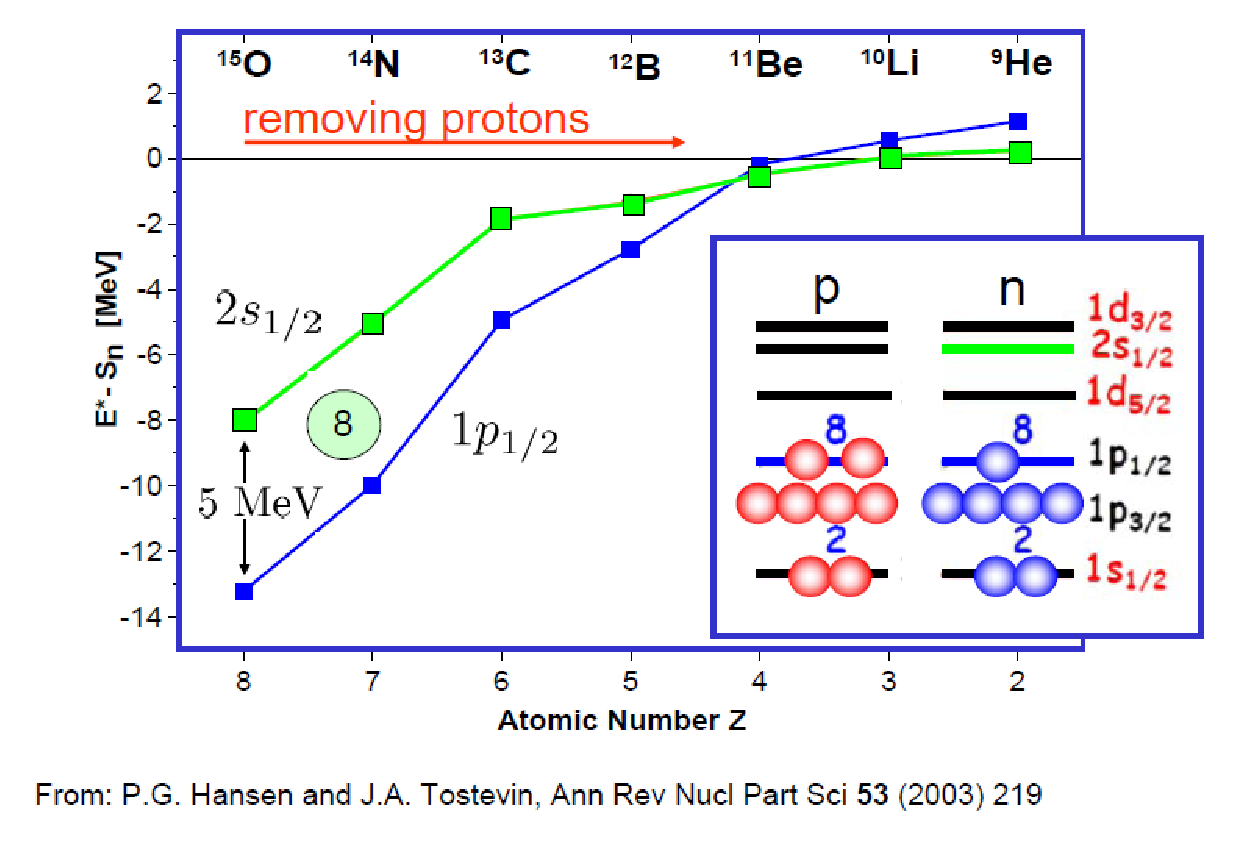
\includegraphics[width=0.95\columnwidth]{\images/n7_sp.eps} \end{center}

\column{0.5\textwidth}
{\verde HP.~Jeppesen et al, PLB642 (2006) 449}

\begin{figure}{\par \resizebox*{0.9\textwidth}{!}
{\includegraphics{\images/bu_vsE_vs100vp67.eps}} \par}
\end{figure}
\end{columns}


% \vspace{-0.25cm}
% \twocolumn{
% \begin{figure}{\par \resizebox*{0.45\textwidth}{!}
% {\includegraphics{10li-trans-cm.eps}} \par}
% \end{figure}
% }{
% %{\verde \em \small We are observing the tail of the proton angular distribution!}
%  }

\end{frame}






\endinput
%%%%%%%%%%%%%%%%%%%%%%%%%%%%%%%%%%%%%%%%%%%%%%%%%% ENDINPUT %%%%%%%%%%%%%%%%%%%%%%%%%%%%%%%%%%%%%%%%%%%%%%%%

% ----------------------------------------------------------------------------------------------------
\slide{Spectroscopic factors: angular momentum considerations}

\begin{itemize}
\setlength{\itemsep}{14pt}
\item We need to evaluate:
$$
\int d\xi \; \phi_a(\xi)  \phi_A (\xi,\br)  \quad \mathrm{and} \quad  \int d\xi' \; \phi_b(\xi')  \phi_B (\xi',\br')  
$$

\item Since $A=a + v$ we can use the parentage decomposition: 
$$
\psframebox[linecolor=red,framearc=0.1]{
\phi_{A}^{JM}(\xi,\br)= \sum_{I\ell j}{\verde C_{IJ}^{\ell sj}} \left[\phi_{a}^{I}(\xi)
\otimes 
 {\verde \varphi_{bv}^{\ell sj}(\br)}\right]_{JM}
}%psfr
$$

\begin{itemize}
\gitem{$\varphi_{bv}^{\ell sj}(\br)$:} wavefunction of the valence particle ($v$) relative to the core $a$. 
\gitem{$C_{IJ}^{\ell sj}$} = spectroscopic amplitudes 
\gitem{$S_{IJ}^{\ell sj}=|C_{IJ}^{\ell sj}|^2$} = spectroscopic factors
\end{itemize}

\bigskip
\pause
%\psframebox[linecolor=blue,framearc=0.1,framesep=0.2]{
\ding{43} {\it The spectroscopic factor gives the probability of finding the nucleon $v$ in the configuration {\red ${\ell sj}$} bound to the core in  the state with spin {\red $I$}.}
%}%psfr

%\item{\blue Target:}
%$\phi_{B}^{J'M'}(\xi',\br')=\sum_{I\ell j}{\brick A_{IJ'}^{\ell sj}} \left[\phi_{b}^{I}(\xi')\otimes\varphi_{\ell sj}(\br')\right]_{J'M'}$
\end{itemize}

\end{frame}



%------------------------------------------------------------
\slide{Adiabatic approximation}
\begin{itemize}
\item For a $(d,p)$ reaction, $\Psi^\mathrm{(+)}_{\bK_d}(\bR,\br)$ is a solution of 
$$
\psframebox[linecolor=red,framearc=0.1]{
[\hat{T}_\bR + H_d(\br) + U_{pb} + U_{nb} - E ] \Psi^\mathrm{(+)}_{\bK_\alpha} =0 
}%psframe
$$

\item  At sufficiently high energies ($E \gg \varepsilon$) we can make the {\blue adiabatic} approximation:
$$
\psframebox[linecolor=red,framearc=0.1]{
H_d (\br) =  \hat{T}_\br + V_{pn}(\br) \simeq \varepsilon_d  
}
$$

\item $\Psi^\mathrm{(+)}_{\bK_d}(\bR,\br) \simeq \Psi^\mathrm{(ad)}_{\bK_d}(\bR,\br) = \chi^{ad}_d(\bR,\br) \varphi_d(\br)$ 
$$
\psframebox[linecolor=red,framearc=0.1]{
[\hat{T}_\bR + \varepsilon_d + U_{pb} + U_{nb} - E]  \chi^{ad}_d(\bR,\br) =0 
}
$$
\ding{43} (still complicated; depends parametrically on $\br$!)
\end{itemize}

\end{frame}




%---------------------------------------------------------
\subsection{Physical example:  $^{56}$Fe(d,p)$^{57}$Fe}
%---------------------------------------------------------
\slide{Transfer example}

{\brick Physical example:} $^{56}$Fe(d,p)$^{57}$Fe at $E_d=12$~MeV

\vspace{2cm}

\begin{columns}
\column{0.5\linewidth}
 \begin{figure}{\par \resizebox*{0.75\textwidth}{!}
 {\includegraphics{\images/fe6dp.eps}} \par}
 \end{figure}
\column{0.5\linewidth}
 \begin{figure}{\par \resizebox*{0.75\textwidth}{!}
 {\includegraphics{\images/fe6dp_dwba.eps}} \par}
 \end{figure}
\end{columns}

\end{frame}



% ------------------------------------------------------------------------------------------------
\slide{Transfer example: $^{56}$Fe(d,p)$^{57}$Fe}

{\brick DWBA scattering amplitude:}

%\vspace{0.5cm}
\begin{center}
$$
\psframebox[linecolor=red,framearc=0.1,framesep=4pt]{
f^\mathrm{DWBA}(\theta)_{i\rightarrow f}=-\frac{\mu_\beta}{2 \pi \hbar^2} C_i C_f \langle\chi_\mathrm{p-^{57}Fe}^{(-)} \phi_\mathrm{^{57}Fe}
|V_\mathrm{prior/post}|
\chi_\mathrm{d-^{56}Fe}^{(+)}\phi_{d}\rangle
}%psframe
$$
\end{center}

\only<2>{
\begin{itemize}
\setlength{\itemsep}{12pt}
\item {\blue $ \chi_\mathrm{d-^{56}Fe}, \chi_\mathrm{p-^{57}Fe}$}: initial and final distorted waves
\item {\blue $\phi_{d}$}: projectile bound wavefunction( $p-n$)
\item {\blue $\phi_\mathrm{^{57}Fe}$}: final (residual) wavefunction (n+\nuc{56}{Fe})
\item {\blue $C_i$, $C_f$}: initial / final spectroscopic amplitudes. 
\item {\blue $V_\mathrm{prior/post}$}: transition potential in PRIOR or POST form
\end{itemize}
}%onslide{2}



% ---------------------
\only<3>{
\begin{columns}
\column{0.5\linewidth}
\begin{center}{\blue PRIOR}\end{center}
\vspace{-0.5cm}
 \begin{figure}{\par \resizebox*{0.38\textwidth}{!}
 {\includegraphics{\images/fe56dp_prior.eps}} \par}
 \end{figure}

$V_\mathrm{prior} = V_\mathrm{n-56Fe}+ \underbrace{U_\mathrm{p-56Fe}-U_\mathrm{d-56Fe}}_\texttt{remnant}$
\column{0.5\linewidth}
\begin{center}{\blue POST}\end{center}
\vspace{-0.5cm}
 \begin{figure}{\par \resizebox*{0.52\textwidth}{!}
 {\includegraphics{\images/fe56dp_post.eps}} \par}
 \end{figure}
$V_\mathrm{post} = V_\mathrm{p-n}+ \underbrace{U_\mathrm{p-56Fe}-U_\mathrm{p-57Fe}}_\texttt{remnant}$
\end{columns} %twocolumn
} %onslide
\end{frame}


% ------------------------------------------------------------------------------------------------




% ------------------------------------------------------------------------------------------------
\slide{Transfer example: $^{56}$Fe(d,p)$^{57}$Fe}


{\bf \brick Essential physical ingredients in a DWBA calculation:}

\bigskip 

\begin{itemize}
  \setlength{\itemsep}{10pt}
\item {\bf \blue  Potentials (5):}
  \begin{itemize}
   \setlength{\itemsep}{8pt}
  \item[$\bullet$] Distorted potential for \underline{entrance} channel (complex): {\verde d+\nuc{56}{Fe}}
  \item[$\bullet$] Distorted potential for \underline{exit} channel (complex):  {\verde p+\nuc{57}{Fe}}
  \item[$\bullet$] Core-core interaction (complex): {\verde p+\nuc{56}{Fe}}
  \item[$\bullet$] Binding potential for projectile (real): {\verde p+n} 
  \item[$\bullet$] Binding potential for target (real): {\verde n+\nuc{56}{Fe}}
  \end{itemize}
\item {\bf \blue Spectroscopic amplitudes:} $C_i$,$C_f$
\end{itemize}
\end{frame}





% ------------------------------------------------------------------------------------------------
\slide
{Transfer example: $^{56}$Fe(d,p)$^{57}$Fe}

{\brick Selectivity of $\ell$:}

\only<1>{
% \begin{example}
%  &OVERLAP (...)  nn=2 l=0 sn=0.5 j=0.5  kbpot=3 be=7.646 /
% &OVERLAP (...)  nn=2 l=1 sn=0.5 j=1.5  kbpot=3 be=7.646 /
% &OVERLAP (...)  nn=2 l=2 sn=0.5 j=2.5  kbpot=3 be=7.646 /
% &OVERLAP (...)  nn=1 l=3 sn=0.5 j=2.5  kbpot=3 be=7.646 /
% &OVERLAP (...)  nn=1 l=4 sn=0.5 j=4.5  kbpot=3 be=7.646 /
%\end{example}
 \begin{figure}{\par \resizebox*{0.55\textwidth}{!}
 {\includegraphics{images/fe56dp_ldep.eps}} \par}
 \end{figure}
}%onslide

\only<2>{
\begin{columns}
\column{0.5\linewidth}
\includegraphics[width=0.9\textwidth]{\images/fe56dp_l0.eps} 
\column{0.5\linewidth}
\includegraphics[width=0.8\textwidth]{\images/fe56dp_l1.eps} 
\end{columns}%twocolumn
{\verde H.M. Sen Gupta et al, Nucl. Phys. A160, 529 (1971)}
}%onslide

\end{frame}




% --------------------------------------------------------------------------------
\slide{DWBA transition amplitude}
\begin{itemize}
\gitem{Using the parentage decompositions for $A$ and $B$:}
$$
\small
\int \Phi^{*}_\beta (\xi_\beta) \Phi_\alpha(\xi_\alpha) \, d\xi d\xi'
=  {\brick C_{IJ}^{\ell sj} C_{I'J'}^{\ell' sj'}}
  \varphi^{\ell' sj'}_{bv}(\br')^{*}  \varphi^{\ell sj}_{av}(\br)   
$$


\gitem{Three-body DWBA transition amplitude}
$$
\psframebox[fillcolor=magenta!8,linecolor=brick,framearc=0.1,fillstyle=solid]{
{\cal T}^\mathrm{DWBA}_{\beta,\alpha} =
%{\red C^B_{vb}  C^A_{va}}
{\red C_{IJ}^{\ell sj} C_{I'J'}^{\ell' sj'}}
 \int \int \chi^{(-)*}_{\beta}(\bK',\bR')  \varphi^{\ell' sj'}_{bv}(\br')^{*}  (V_\beta- U_\beta) 
   \chi_{\alpha}^{(+)}(\bK,\bR)  \varphi^{\ell sj}_{av}(\br) d\bR' d\br' 
}%
$$

\gitem{Differential cross section:} 
% See Glendenning Eq. (5.50)
\small
$$
\psframebox[linecolor=brick,framearc=0.1,framesep=1pt,fillcolor=magenta!8,fillstyle=solid]{
\frac{d\sigma_{\alpha,\beta}}{d\Omega} = 
\frac{\mu_\alpha \mu_\beta}{(2 \pi \hbar^2)^2}  {\red S_{IJ}^{\ell sj} S_{I'J'}^{\ell' sj'}} 
{K_f \over K_i}
\left|  \int \int \chi^{(-)*}_{\beta}(\bK',\bR')  \varphi^{\ell' sj'}_{bv}(\br')^{*}   (V_\beta- U_\beta) 
   \chi_{\alpha}^{(+)}(\bK,\bR)  \varphi^{\ell sj}_{av}(\br) d\bR' d\br' 
\right|^2
}%psframebox
$$

\item[\ding{43}] {\em \blue \small In DWBA, the transfer cross section is proportional to the product  $S_{IJ}^{\ell sj} S_{I'J'}^{\ell' sj'}$}
\end{itemize}

\end{frame}




\endinput


%-----------------------------------------------------------------------------------------------------
\subsection{Advanced topic: The Coupled-Reaction Channels formalism}


\slide{}
\begin{center}
\psframebox[fillcolor=green!10,linecolor=blue,framearc=0.1,fillstyle=solid,framesep=5pt]{
Advanced topic: Coupled-Reaction Channels method
}%psframe
\end{center} 
\end{frame}



\subsection{Extra stuff...}



% ----------------------------------------------------------------------------------------------------
\slide{Brief summary on transfer reactions}

\begin{itemize}
\setlength{\itemsep}{12pt}

\gitem{Inclusion of transfer couplings in the Schrodinger equation gives rise to a set of coupled equations with 
non-local kernels (Coupled Reactions Channels)}

\gitem{If transfer couplings are weak, the CRC equations can be solved in Born approximation $\Rightarrow$ DWBA approximation}

\gitem{The DWBA amplitude is proportional to the product of the projectile and target spectroscopic factors.}

\gitem{The analysis of transfer reactions provide information on:}
\begin{itemize} 
\item Spectroscopic factors.
\item Quantum number for single-particle configurations ($n,\ell,j$).
\item Binding interactions.
\item Reactions mechanisms.
\end{itemize}

\end{itemize}
\end{frame}



%%%%%%%%%%%%%%%%%%%%%%%%%%%%%%%%%%%%%%%%%%%%%%%%%%%%%%%%%%%%%%%%%%%%%%%%%%%%%%%%%%%%%%%%%%%%%%%%%%%%
\endinput

%---------------------------------------------------------------
\slide{Evaluation of scattering amplitude in Born approximation}
\begin{itemize}
\item Define auxiliary potentials in entrance ($\alpha=d$) and exit $\beta=p$) channels: 
% $U_\alpha(\bR_\alpha)$, $U_\beta(\bR_\beta)$ 
\begin{align*}
\left[E_d-\hat{T}_{\bR_\alpha}-U_{\alpha}(\bR_\alpha) \right] \chi^{(+)}_{\alpha}(\bK_\alpha,\bR_\alpha) & =  0 \\
\left[E_p-\hat{T}_{\bR_\beta}-U_{\beta}(\bR_\beta) \right] \chi^{(+)}_{\beta}(\bK_\beta,\bR_\beta) & =  0
\end{align*}

\item Retain only elastic component of $\Psi^\mathrm{(+)}_{\bK_\alpha}$  ({\blue Born approximation}):
$$
\Psi^\mathrm{(+)}_{\bK_\alpha} (\bR_\alpha,\xi_\alpha) \approx \chi^{(+)}_{\alpha}(\bK_\alpha,\bR_\alpha) \Phi_\alpha(\xi_\alpha)
$$

\item DWBA scattering amplitude:
$$
\psframebox[fillcolor=magenta!8,linecolor=brick,framearc=0.1,fillstyle=solid]{
{\cal T}^\mathrm{DWBA}_{\beta,\alpha} = 
\int \int \chi_{\beta}^{(-)*}(\bK_\beta, \bR_\beta) 
  \Phi^{*}_\beta (\xi_\beta) (V_\beta-U_\beta)    \chi^{(+)}_{\alpha}(\bK_\alpha,\bR_\alpha) \Phi_\alpha(\xi_\alpha) d\xi_\beta d\bR_\beta 
}%psframe
$$
\end{itemize}
\end{frame}




\slide{}
\only<1,2>{
\begin{itemize}
\gitem{We seek for the differential cross section:}
$$
  \frac{d\sigma_{if}(\theta)}{d\Omega} = \frac{K_f}{K_i}  \left|{\red f_{f,i}(\theta)} \right|^2
$$
\gitem{For {\blue inelastic excitations} and within the {\blue DWBA} approximation:}

$$
\psframebox[fillcolor=yellow,linecolor=red,framearc=0.1]{
f(\mathbf{K'},\mathbf{K})_{f,i}=-\frac{\mu}{2 \pi \hbar^2} \int d\bR \widetilde{\chi}_{f}^{(-)*}(\bK',\bR) V_{fi}(\bR) \widetilde{\chi}_{i}^{(+)}(\bK,\bR)
}%psframebox
$$
\end{itemize}
}%onslide

\only<2>{ 
with
\begin{itemize}
\gitem{$\widetilde{\chi}_{i}^{(+)}(\bK,\bR)$, $\widetilde{\chi}_{f}^{(-)}(\bK',\bR)$}:  distorted waves  describing the projectile-motion in the initial ($i$) or final ($f$)  state.
%\gitem{$\widetilde{\chi}_{f}^{(-)}(\bK',\bR)$}: distorted wave that describes the projectile-motion in the final state.
\gitem{$V_{fi}(\bR)$} coupling potentials:
$$
\psframebox[linecolor=red,framearc=0.1]{
V_{f,i}(\bR) = \int   d \xi \phi_{f}(\xi)^* V(\bR, \xi) \phi_{i}(\xi) 
}%psframebox
$$
\end{itemize}
}%onslide1
\end{frame}














